\documentclass[oneside]{book}
\usepackage{ctex}
\usepackage{amssymb}
\usepackage[hidelinks]{hyperref}
\usepackage{amsthm}
\usepackage{graphicx}
\title{MIT 18.01}
\author{Lyshmily.Y}
\date{\today}
\begin{document}
	\maketitle
	\tableofcontents
	\newpage
	\chapter{导数和变化率}
	\textbf{微分}
	
	1.几何解释
	
	如何求某图像某点处的切线?例如函数$y=f(x)$在点$P(x_{0},y_{0})$处切线方程为:\ $y-y_{0}=m(x-x_{0})$,其中$y_{0}=f(x_{0})$,要想确定切线的方程,我们必须知道$m$的值;我们令$m=f^{'}(x_{0})$,我们定义$f(x)$在$x=x_{0}$处的导数$f^{'}(x_{0})$为函数$y=f(x)$在此点处切线的斜率.
	
	我们换一种方式来看切线:假设函数有一条割线$l$,与函数图像交于$P,Q$两点,当点$Q$不断接近于点$P$时,$l$称为函数在点$P$处的切线,切线就可以看作是割线$PQ$的极限.由此我们假设$Q$点坐标$(x_{0}+\Delta x,f(x_{0}+\Delta x))$,割线$PQ$的斜率$k_{PQ}=\frac{f(x_{0}+\Delta x)-f(x_{0})}{\Delta}$;因此切线的斜率:
	$$m=\lim\limits_{\Delta x\rightarrow 0}(\frac{f(x_{0}+\Delta x)-f(x_{0})}{\Delta x})\Rightarrow m=f^{'}(x_{0})$$
	
	我们来看一个简单的例子:
	$f(x)=\frac{1}{x}$,求$f(x)$的导数,根据函数切线斜率定义:$$f^{'}(x_{0})=\lim\limits_{\Delta x\rightarrow 0}(\frac{f(x_{0}+\Delta x)-f(x_{0})}{\Delta x})=\lim\limits_{\Delta x\rightarrow 0}(\frac{\frac{1}{x_{0}+\Delta x}-\frac{1}{x_{0}}}{\Delta x})$$
	\centerline{$\Updownarrow$}
	$$\lim\limits_{\Delta x\rightarrow 0}(\frac{-1}{x_{0}^{2}+x_{0}\Delta x})$$
	$$f^{'}(x_{0})=-\frac{1}{x_{0}^{2}}$$
	当$x_{0}\rightarrow 0$时,函数图像越陡峭;当$x_{0}\rightarrow \infty$时,函数图像越平缓.
	
	我们进一步提出一个问题:如何求$f(x)=\frac{1}{x}$切线与坐标轴围成的面积.
	
	根据上一个例子,我们知道函数在点$P(x_{0},\frac{1}{x_{0}})$处切线斜率$k_{P}=-\frac{1}{x_{0}^{2}}$,切线方程为$y-\frac{1}{x_{0}}=-\frac{1}{x_{0}^{2}}(x-x_{0})$,假设切线与$x,y$轴相交于$A,B$两点,我们得到$A(2x_{0},0),B(0,\frac{2}{x_{0}})$,$S_{\Delta AOB}=\frac{1}{2}|OA|*|OB|=2$.
	
	2.导数表示方法:
	
	(1).$y=f(x)$,$f^{'}(x)=\lim\limits_{\Delta x\rightarrow 0}\frac{\Delta y}{\Delta x}=\lim\limits_{\Delta x\rightarrow 0}\frac{\Delta f}{\Delta x}$
	
	(2).$y=f(x)$的导数可以写作$y^{'},f^{'}(x)$,$\frac{\mathrm{d}f}{\mathrm{d}x}$,$\frac{\mathrm{d}y}{\mathrm{d}x}$,$\frac{\mathrm{d}}{\mathrm{d}x}f$,$\frac{\mathrm{d}}{\mathrm{d}x}y$.
	
	\hspace{\fill}\
	
	下一个例子是:求$y=x^{n}$的导数.
	
	$y^{'}=\lim\limits_{\Delta x\rightarrow 0}\frac{(x+\Delta x)^{n}-x^{n}}{\Delta x}$,我们由二项展开式$(x+\Delta x)^{n}=x^{n}+nx^{n-1}\Delta x+...+(\Delta x)^{n}\rightarrow (x+\Delta x)^{n}=x^{n}+nx^{n-1}\Delta x+O(\Delta x)$;因此我们得到:$$y^{'}=\lim\limits_{\Delta x\rightarrow 0}(\frac{nx^{n-1}\Delta x+O(\Delta x)}{\Delta x}=nx^{n-1}$$
	
	3.物理解释
	
	在物理学中有许多通过比值定义的物理量,比如速度;我们在实际生活中将$\frac{\Delta s}{\Delta t}$称为物体在$\Delta t$内的平均速度,当$\Delta t\rightarrow 0$时,$\lim\limits_{\Delta t\rightarrow 0}\frac{\Delta s}{\Delta t}$称为物体在某一点处的瞬时速度,也被称为函数在该点处的导数.
	
	我们来看另一个很好的例子,卫星的$GPS$定位,假设基站和卫星距离为$H$,人和卫星的距离为$L$,基站和人的距离为$S$,我们发现误差系数$\frac{\Delta S}{\Delta L}=\frac{\mathrm{d}S}{\mathrm{d}L}$.
	
	\chapter{极限和连续}
	
	\centerline{{\large \textbf{极限}}}
	
	\textbf{例子和定义}
	
	1.简单极限
	
	形如:$\lim\limits_{x\rightarrow 4}\frac{2x1}{x^{2}+1}=\frac{7}{17}$.
	
	2.导数
	
	假设函数$f(x)$在$x=x_{0}$处导数存在,$f^{'}(x_{0})=\lim\limits_{x\rightarrow x_{0}}\frac{f(x)-f(x_{0})}{x-x_{0}}$
	
	3.序列极限
	
	假设有数列$\left\lbrace a_{n}\right\rbrace$,\ $\exists A >0,\ \exists N_{0}>0$,对于$\forall \varepsilon >0$,当$n>N_{0}$时满足$|a_{n}-A|<\varepsilon$,我们称序列$\left\lbrace a_{n} \right\rbrace $的极限为$A$;我们可以写作:
	$$\lim\limits_{n\rightarrow +\infty}a_{n}=A\ or\ \lim\limits_{n\rightarrow +\infty}(a_{n}-A)=0 $$ 
	
	4.函数极限
	
	(1).函数在$x=x_{0}$处极限
	
	对于$\forall\varepsilon >0$,\ $\exists\delta>0$当$0<|x-x_{0}|<\delta$时,都有$|f(x)-A|<\varepsilon$,我们称$f(x)$在$x=x_{0}$处的极限为$A$;我们写作:
	$$\lim\limits_{x\rightarrow x_{0}}f(x)=A\ or\ \lim\limits_{x\rightarrow x_{0}}(f(x)-A)=0$$ 
	\textbf{注意}:左右极限必须相等
	
	(2).函数在无穷远处极限
	
	对于$\forall\varepsilon >0$,$\exists X>0$,当$x>X$时,都有$|f(x)-A|<\varepsilon$,我们称$f(x)$在$+\infty$处的极限为$A$;我们写作:
	$$\lim\limits_{x\rightarrow +\infty}f(x)=A\ or\ \lim\limits_{x\rightarrow +\infty}(f(x)-A)=0$$
	对于$\forall\varepsilon >0$,$\exists X<0$,当$x<X$时,都有$|f(x)-A|<\varepsilon$,我们称$f(x)$在$-\infty$处的极限为$A$;我们写作:
	$$\lim\limits_{x\rightarrow -\infty}f(x)=A\ or\ \lim\limits_{x\rightarrow -\infty}(f(x)-A)=0$$
	\textbf{左右极限}
	
	极限分为左极限和右极限,极限存在当且仅当左极限等于右极限;函数在某个点处的极限和该点处函数值无关.
	$$Left\ Limit \lim\limits_{x\rightarrow x_{0}^{-}}f(x)$$
	$$Right\ Limit\lim\limits_{x\rightarrow x_{0}^{+}}f(x) $$
	函数在某点处极限存在,我们得到:
	$$\lim\limits_{x\rightarrow x_{0}^{-}}f(x)=\lim\limits_{x\rightarrow x_{0}^{+}}f(x)$$
	\centerline{{\large \textbf{连续}}}
	
	\textbf{定义}
	
	$f(x)$在$x=x_{0}$处连续$\Leftrightarrow\lim\limits_{x\rightarrow x_{0}}f(x)=f(x_{0})$
	
	\textbf{定理}:函数可导必连续,连续不一定可导.
	\begin{proof}
		我们需要证明:$\lim\limits_{x\rightarrow x_{0}}f(x)-f(x_{0})=0$
		
		$$\lim\limits_{x\rightarrow x_{0}}f(x)-f(x_{0})\Leftrightarrow \lim\limits_{x\rightarrow x_{0}}\frac{f(x)-f(x_{0})}{x-x_{0}}(x-x_{0})$$根据函数在此点处可导得到:$\lim\limits_{x\rightarrow x_{0}}\frac{f(x)-f(x_{0})}{x-x_{0}}$存在,且$\lim\limits_{x\rightarrow x_{0}}(x-x_{0})=0$,因此我们得到:
		$$\lim\limits_{x\rightarrow x_{0}}f(x)-f(x_{0})=f^{'}(x_{0})*0=0$$
	\end{proof}
	\hspace{\fill}\
	
	\centerline{{\large \textbf{间断}}}
	
	1.第一类间断点
	
	(1).可去间断点
	
	$Left\ Limit=Right\ Limit$时,$\lim\limits_{x\rightarrow x_{0}^{-}}f(x)=\lim\limits_{x\rightarrow x_{0}^{+}}f(x)$,被称为可去间断点.
	
	例如:函数$f(x)=\frac{\sin x}{x}$在$x=0$处是可去间断点,$\lim\limits_{x\rightarrow 0}\frac{\sin x}{x}=1$;函数$f(x)=\frac{1-\cos x}{x}$在$x=0$处是可去间断点,$\lim\limits_{x\rightarrow 0}\frac{1-\cos x}{x}=0$.
	
	
	(2).跳跃间断点
	
	$Left\ Limit\neq Right\ Limit$时,$\lim\limits_{x\rightarrow x_{0}^{-}}f(x)\neq\lim\limits_{x\rightarrow x_{0}^{+}}f(x)$,被称为跳跃间断点.
	
	2.第二类间断点
	
	左极限和右极限至少有一个不存在.
	
	\textbf{重要极限}:使用几何证明法
	\begin{equation}
		\lim\limits_{x\rightarrow 0}\frac{\sin x}{x}=1
	\end{equation}
	\begin{equation}
		\lim\limits_{x\rightarrow 0}\frac{1-\cos x}{x}=0
	\end{equation}
	
	\chapter{求导四则运算及三角函数导数}
	\textbf{求导法则}
	
	1.三角函数求导
	
	$\frac{\mathrm{d}}{\mathrm{d}x}\sin x=\cos x$;\ $\frac{\mathrm{d}}{\mathrm{d}x}\cos x=-\sin x$
	
	(1).$$\lim\limits_{\Delta x\rightarrow 0}\frac{\sin(x+\Delta x)-\sin x}{\Delta x}\Leftrightarrow \lim\limits_{\Delta x\rightarrow 0}(\sin x\frac{\cos\Delta x-1}{\Delta x}+\cos x\frac{\sin \Delta x}{\Delta x})$$由公式$(2.1)$和$(2.2)$得到$\lim\limits_{\Delta x\rightarrow 0}\frac{\sin(x+\Delta x)-\sin x}{\Delta x}=\cos x$.
	
	(2).$$\lim\limits_{\Delta x\rightarrow 0}\frac{\cos(x+\Delta x)-\cos x}{\Delta x}\Leftrightarrow \lim\limits_{\Delta x\rightarrow 0}(\cos x\frac{\cos\Delta x-1}{\Delta x}-\sin x\frac{\sin \Delta x}{\Delta x})$$由公式$(2.1)$和$(2.2)$得到$\lim\limits_{\Delta x\rightarrow 0}\frac{\cos(x+\Delta x)-\cos x}{\Delta x}=-\sin x$.
	
	2.求导四则运算
	
	(1).$(f(x)\pm g(x))^{'}=f^{'}(x)\pm g^{'}(x)$
	
	(2).$(Cf(x)))^{'}=Cf^{'}(x)$
	
	(3).$(f(x)g(x))^{'}=f^{'}(x)g(x)+f(x)g^{'}(x)$
	\begin{proof}
		\begin{equation}
		\lim\limits_{\Delta x\rightarrow 0}\frac{f(x+\Delta x)g(x+\Delta x)-f(x)g(x)}{\Delta x}
	\end{equation}
	\centerline{$\Updownarrow$}
	\begin{equation}
		\lim\limits_{\Delta x\rightarrow 0}\frac{(f(x+\Delta x)-f(x))g(x+\Delta x)+f(x)g(x+\Delta x)-f(x)g(x)}{\Delta x}
	\end{equation}
	\centerline{$\Updownarrow$}
	\begin{equation}
	 \lim\limits_{\Delta x\rightarrow 0}\frac{(f(x+\Delta x)-f(x))g(x+\Delta x)+f(x)(g(x+\Delta x)-g(x))}{\Delta x}
	\end{equation}
	\end{proof}	
	后面的式子可以写作:$$\lim\limits_{\Delta x\rightarrow 0}(\frac{f(x+\Delta x)-f(x)}{\Delta x})g(x+\Delta x)*(\frac{g(x+\Delta x)-g(x)}{\Delta x})(f(x))$$,根据极限的运算法则,这个式子可以写作$f^{'}(x)g(x)+f(x)g^{'}(x)$.
	
	(4).$(\frac{f(x)}{g(x)})^{'}=\frac{f^{'}(x)g(x)+f(x)g^{'}(x)}{g^{2}(x)}$
	\begin{proof}
		\begin{equation}
		\lim\limits_{\Delta x\rightarrow 0}\frac{\frac{f(x+\Delta x)}{g(x+\Delta x)}-\frac{f(x)}{g(x)}}{\Delta x}
		\end{equation}
	\centerline{$\Updownarrow$}
		\begin{equation}
		\lim\limits_{\Delta x\rightarrow 0}\frac{f(x+\Delta x)g(x)-g(x+\Delta x)f(x)}{\Delta xg(x)g(x+\Delta x)}
		\end{equation}
	\centerline{$\Updownarrow$}
		\begin{equation}
		\lim\limits_{\Delta x\rightarrow 0}\frac{f(x+\Delta x)g(x)-g(x+\Delta x)f(x)}{\Delta x}*\frac{1}{g(x)g(x+\Delta x)}
		\end{equation}		
		由$(3.1),(3.2),(3.3)$得到结果为$\frac{f^{'}(x)g(x)-f(x)g^{'}(x)}{g^{2}(x)}$.
	\end{proof}
	\chapter{链式法则及高阶导数}
	\centerline{\textbf{链式法则}}
	
	$y=f(t),t=g(x)$,$\frac{\mathrm{d}y}{\mathrm{d}x}=\frac{\mathrm{d}y}{\mathrm{d}t}*\frac{\mathrm{d}t}{\mathrm{d}x}=f^{'}g^{'}$
	
	\centerline{\textbf{高阶导数}}
	函数$y=f(x)$的$n$阶导数为$y^{(n)}=f^{n}(x)$;当然我们还可以换个写法:
	\begin{equation}
		y^{(n)}=f^{n}(x)=\frac{\mathrm{d}^{n}y}{\mathrm{d}x^{n}}
	\end{equation}
	我们来看一个例子:$y=x^{n}$的$m$阶导数$(m<n)$:
	$$y^{(n)}=\frac{n!}{(n-m)!}x^{n-m}$$
	\chapter{隐函数微分法和反函数导数}
	\textbf{隐函数微分法}
	
	我们来看几个例子:
	
	1.$y=x^{\frac{m}{n}}$
	
	这个式子等价于$y^{n}=x^{m}$,我们看出这是一个隐函数,我们可以使用隐函数微分法解决这个问题,对上面的式子左右两边对$x$求导:
	$$\frac{\mathrm{d}y^{n}}{\mathrm{d}x}=mx^{m-1}\Rightarrow ny^{n-1}\frac{\mathrm{d}y}{\mathrm{d}x}=mx^{m-1}$$
	
	因此我们得到:$\frac{\mathrm{d}y}{\mathrm{d}x}=\frac{m}{n}x^{\frac{m}{n}-1}$.
	
	2.$x^{2}+y^{2}=1$
	
	同样的我们知道$y=f(x)$,我们对上面式子左右对$x$求导,得到:
	$$2x+2y\frac{\mathrm{d}y}{\mathrm{d}x}=0\Rightarrow \frac{\mathrm{d}y}{\mathrm{d}x}=\frac{-x}{y}$$
	
	我们发现我们并没有解出完整的导数,但是我们只需要知道$(x_{0},f(x_{0}))$,我们就能知道该点处切线的斜率、导数,这是我们使用隐函数微分的目的,大大简化我们的过程.
	
	3.$y^{4}+xy^{2}-2=0$
	
	我们对式子两边同时对$x$求导:$$4y^{3}\frac{\mathrm{d}y}{\mathrm{d}x}+y^{2}+2xy\frac{\mathrm{d}y}{\mathrm{d}x}=0\Rightarrow \frac{\mathrm{d}y}{\mathrm{d}x}=\frac{-y^{2}}{4y^{3}+2xy}$$
	\textbf{反函数导数}
	
	原函数$y=f(x)$和反函数$x=g(y)$满足$\left\{\begin{array}{c}
		f(g(y))=y\\g(f(x))=x
	\end{array}\right.$.\ 那么我们有$f=g^{-1},g=f^{-1}$.原函数的定义域为反函数的值域,原函数的值域为反函数的定义域.

	如何求反函数导数?
	
	我们通常采用隐函数求导的方法去求反函数的导数,我们可以举出两个比较典型的例子,比如$y=\tan(x),\ x\in (-\frac{\pi}{2},\frac{\pi}{2})$和$y=\sin(x),\ x\in (-\frac{\pi}{2},\frac{\pi}{2})$的反函数:反正切函数\ $y=\arctan x$\ 和反正弦函数\ $y=\arcsin x$
	
	反正切函数:$\tan y=x$,我们对式子两边对$x$求导得到:
	$$\frac{1}{\cos^{2}y}\frac{\mathrm{d}y}{\mathrm{d}x}=1\Rightarrow \frac{\mathrm{d}y}{\mathrm{d}x}=\cos^{2}y$$
	我们构造一个直角三角形,有一个角$\theta=y,y\ \in (-\infty,+\infty)$满足$tan y=x,x \in (-\frac{\pi}{2},\frac{\pi}{2})$,那么这个直角三角形中$\theta$对应的边为$x$,另一条直角边为$1$,斜边长为$\sqrt{1+x^{2}}$,因此我们得到:$\cos y=\frac{1}{\sqrt{1+x^{2}}}$,所以反正切函数的导数:$$\frac{\mathrm{d}y}{\mathrm{d}x}=\frac{1}{1+x^{2}}$$
	
	反正弦函数:$\sin y=x$,和上面的做法类似,我们得到$\frac{\mathrm{d}y}{\mathrm{d}x}=\frac{1}{\cos y}$.
	
	我们同样构造一个直角三角形有一个角$\theta=y,y\ \in (-1,1)$满足$\sin y=x,x\in (-\frac{\pi}{2},\frac{\pi}{2})$,在这个直角三角形中$\theta$对应的直角边为$x$,斜边长为$1$,因此$\cos y=\sqrt{1-x^{2}}$,所以反正弦函数的导数:$$\frac{\mathrm{d}y}{\mathrm{d}x}=\frac{1}{\sqrt{1-x^{2}}}$$
	\chapter{指数与对数函数导数、对数微分法}
	\centerline{\textbf{指数函数}}
	
	函数$y=a^{x},(a>0 \and\ a\neq 1)$为指数函数,我们来求这个函数的导函数:
	$$\frac{\mathrm{d}y}{\mathrm{d}x}=\lim\limits_{\Delta x\rightarrow 0}\frac{a^{x+\Delta x}-a^{x}}{\Delta x}$$
	\centerline{$\Updownarrow$}
	$$\frac{\mathrm{d}y}{\mathrm{d}x}=\lim\limits_{\Delta x\rightarrow 0}a^{x}\frac{a^{\Delta x}-1}{\Delta x}$$
	\centerline{$\Updownarrow$}
	$$\frac{\mathrm{d}y}{\mathrm{d}x}=a^{x}\lim\limits_{\Delta x\rightarrow 0}\frac{a^{\Delta x}-1}{\Delta x}=a^{x}\left.\frac{\mathrm{d}y}{\mathrm{d}x}\right|_{x=0}=a^{x}M(a)$$
	
	我们定义$a=e$时满足$M(e)=1$,此时当$y=e^{x}$时我们有: \begin{equation}
	\frac{\mathrm{d}y}{\mathrm{d}x}=e^{x}\end{equation}如何说明我们定义的$e$是存在的呢?
	
	我们假设$f(x)=2^{x}$,$f^{'}(0)=M(2)$,那么对于函数$g(x)=f(kx)=2^{kx}$而言,$g^{'}(x)=f^{'}(kx)=kf^{'}(kx)$,所以$g^{'}(0)=kM(2)$,总能找到一个$k=\frac{1}{M(2)}$,使得$g^{'}(0)=1$,此时$b=2^{k}=e$存在.
	
	假设有函数$y=e^{x}$,关于这个函数的反函数$e^{y}=x$的导数,我们采用隐函数微分的方法来求,对式子左右对$x$求导,根据$(6.1)$得:
	$$\frac{\mathrm{d}e^{y}}{x}=1\Rightarrow e^{y}\frac{\mathrm{d}y}{\mathrm{d}x}=1\Rightarrow \frac{\mathrm{d}y}{\mathrm{d}x}=\frac{1}{x}$$
	
	我们将函数$y=e^{x}$的反函数记作$y=\ln x$,称作对数函数,而且我们有:\begin{equation}
		\frac{\mathrm{d}y}{\mathrm{d}x}=\frac{1}{x}
	\end{equation}
	由$(6.1),(6.2)$两个式子和$e$的定义,我们可以得到一般指数函数的求导公式:$$\frac{\mathrm{d}y}{\mathrm{d}x}=\frac{\mathrm{d}a^{x}}{\mathrm{d}x}=\frac{\mathrm{d}e^{x\ln a}}{\mathrm{d}x}=\ln a (e^{x\ln a})=a^{x}\ln a$$.
	
	\centerline{\textbf{对数函数}}
	
	我们有一般指数函数$y=a^{x}$,它的反函数记作$a^{y}=x$,我们将其记作$y=\log_{a}x$,特别的,当$a=e$时,我们将其记作$y=\ln x$,\ $e$也被称为自然对数.
	
	我们已经知道$(\ln x)^{'}=\frac{1}{x}$,如何去求一般的对数函数的导数?
	
	对于函数$y=\log x\Leftrightarrow a^{y}=x$,我们仍然利用隐函数微分法,可以得到:
	$$a^{y}\ln a\frac{\mathrm{d}y}{\mathrm{d}x}=1\Rightarrow \frac{\mathrm{d}y}{\mathrm{d}x}=\frac{1}{x\ln a}$$
	
	至此我们已经得到了关于指数和对数函数的求导法则:
	$$\frac{\mathrm{d}a^{x}}{\mathrm{d}x}=a^{x}\ln a,\ When \ a=e, \frac{\mathrm{d}e^{x}}{\mathrm{d}x}=e^{x}$$
	$$\frac{\mathrm{d}\log_{a}x}{\mathrm{d}x}=\frac{1}{x\ln x},\ When\ a=e,\ \frac{\mathrm{d}\ln x}{\mathrm{d}x}=\frac{1}{x}$$
	
	\hspace{\fill}\
	
	我们来看一个很经典的例子:$\lim\limits_{n\rightarrow +\infty}(1+\frac{1}{n})^{n}$
	
	假设极限存在,我们不妨将其记作$A$,我们有$\lim\limits_{n\rightarrow +\infty}\ln((1+\frac{1}{n})^{n})=\ln A$,化简得到$\lim\limits_{n\rightarrow +\infty}n\ln((1+\frac{1}{n}))=\ln A$,我们令$\Delta x=\frac{1}{n}$,上面的极限表达式等价于$\lim\limits_{\Delta x\rightarrow 0}\frac{\ln(1+\Delta x)-\ln 1}{\Delta x}=\left.\frac{\mathrm{d}\ln x}{\mathrm{d}x}\right|_{x=1}=1$,因此$\ln A=1\Rightarrow A=e$.我们得到了我们一开始定义的$e$的数值表达式,即:$$e=\lim\limits_{n\rightarrow +\infty}(1+\frac{1}{n})^{n}\approx 2.71828$$
	\chapter{线性和二阶近似}
	\centerline{\textbf{线性近似}}
	函数在某一点处附近近似于该点处的切线,表达式是如下:
	$$f(x)\approx f(x_{0})+f^{'}(x_{0})(x-x_{0})$$
	表示在$x=x_{0}$附近可以将函数近似看作一个线性函数.我们来看几个例子:$y=\sin x,y=\cos x,y=\ln (x-1),y=e^{x},y=(1+x)^{r}$这几个函数在$x=0$附近的线性近似.
	
	当$\delta>0$很小时,$\forall x\in\ (-\delta,\delta)$,我们有\begin{equation}\left\{\begin{array}{c}
		\sin x\approx x\\\cos x\approx 1\\\ln(x-1)\approx x\\e^{x}\approx x+1\\(1+x)^{r}\approx 1+rx
	\end{array}\right.\end{equation}
	
	\centerline{\textbf{二阶近似}}
	
	二阶近似是在线性近似的基础上进一步的精确结果,表达式如下:
	$$f(x)\approx f(x_{0})+f^{'}(x_{0})x+\frac{f^{''}(x_{0})}{2}x^{2}$$
	我们由$(7.1)$可以得到下面的二阶近似结果:
	
	当$\delta>0$很小时,$\forall x\in\ (-\delta,\delta)$,我们有
	\begin{equation}\left\{\begin{array}{c}
			\sin x\approx x\\\cos x\approx 1-\frac{x^{2}}{2}\\\ln(x-1)\approx x-\frac{x^{2}}{2}\\e^{x}\approx 1+x+\frac{x^{2}}{2}\\(1+x)^{r}\approx 1+rx+\frac{r(r-1)}{2}x^{2}
		\end{array}\right.\end{equation}
	我们来看一个例子:$f(x)=e^{-3x}(1+x)^{-\frac{1}{2}}$的二阶近似表达式
	
	我们知道$e^{-3x}\approx 1-3x-\frac{9}{2}x^{2}$;\ $(1+x)^{-\frac{1}{2}}\approx 1-\frac{1}{2}x+\frac{3}{8}x^{2}$.
	
	$f(x)\approx (1-3x-\frac{9}{2}x^{2})(1-\frac{1}{2}x+\frac{3}{8}x^{2})\approx 1-\frac{7}{2}x+\frac{51}{8}x^{2}+O(x^{2})$
	\chapter{曲线构图}
	
	1.\textbf{函数单调性和导数关系}
	
	对于函数$y=f(x)$在$(a,b)$上连续且二阶可导,函数单调性和导数的关系为:
	
	(1).$f^{'}(x)>0$,$f(x)$在$(a,b)$上单调递增;$f^{'}(x)<0$,$f(x)$在$(a,b)$上单调递减.
	
	(2).$f^{''}(x)>0$,$f^{'}(x)$在$(a,b)$上单调递增;$f^{''}(x)<0$,$f^{'}(x)$在$(a,b)$上单调递减.
	
	(3).$f^{''}(x)>0$,$f(x)$是凹函数(Concave\ Up);\ $f^{''}(x)<0$,$f(x)$是凸函数(Concave\ Down).
	
	2.\textbf{作出函数图像}
	
	我们只需要根据函数的导函数求出函数的单调区间和极值,根据函数的二阶导函数看出函数的凸凹性质.
	
	(1).描点,找出特殊点,比如和坐标轴交点;无穷远处函数趋近值.
	
	(2).令$f^{'}(x)=0$,求出函数的驻点.
	
	(3).根据导函数判断函数的单调区间、单调性和极值.
	
	(4).根据二阶导数判断函数的凸凹性.
	
	(5).用平滑的曲线连接所描的点.
	
	3.\textbf{极值和驻点}
	
	对于$f^{'}(x_{0})=0$的点$(x_{0},f(x_{0}))$称为$f(x)$的驻点,对于很小的$\delta>0$,满足$f^{'}(x_{0}-\delta)f^{'}(x_{0}+\delta)<0$的驻点被称为函数$f(x)$的极值点.我们有极值点一定是驻点,但是驻点不一定是极值点.
	
	当$f^{'}(x_{0}-\delta)<0,\ f^{'}(x_{0}+\delta)>0$,$f(x_{0})$是$f(x)$的极小值,$x=x_{0}$是$f(x)$的极小值点;当$f^{'}(x_{0}-\delta)>0,\ f^{'}(x_{0}+\delta)<0$,$f(x_{0})$是$f(x)$的极大值,$x=x_{0}$是$f(x)$的极大值点.
	
	我们举了一个简单的例子:$f(x)=3x-x^{3}$.
	
	$f^{'}(x)=3(1-x)(1+x)$,$x\in\ (-\infty,-1),f^{'}(x)<0;x\in\ (-1,1),f^{'}(x)>0;x\in\ (1,+\infty),f^{'}(x)<0$.
	
	$f^{''}(x)=-6x$,$x\in\ (-\infty,0),f^{''}>0,\ x\in\ (0,+\infty),f^{''}<0$.$f(x)$图像如下图所示.
	\begin{figure}[htbp]
		\centering
		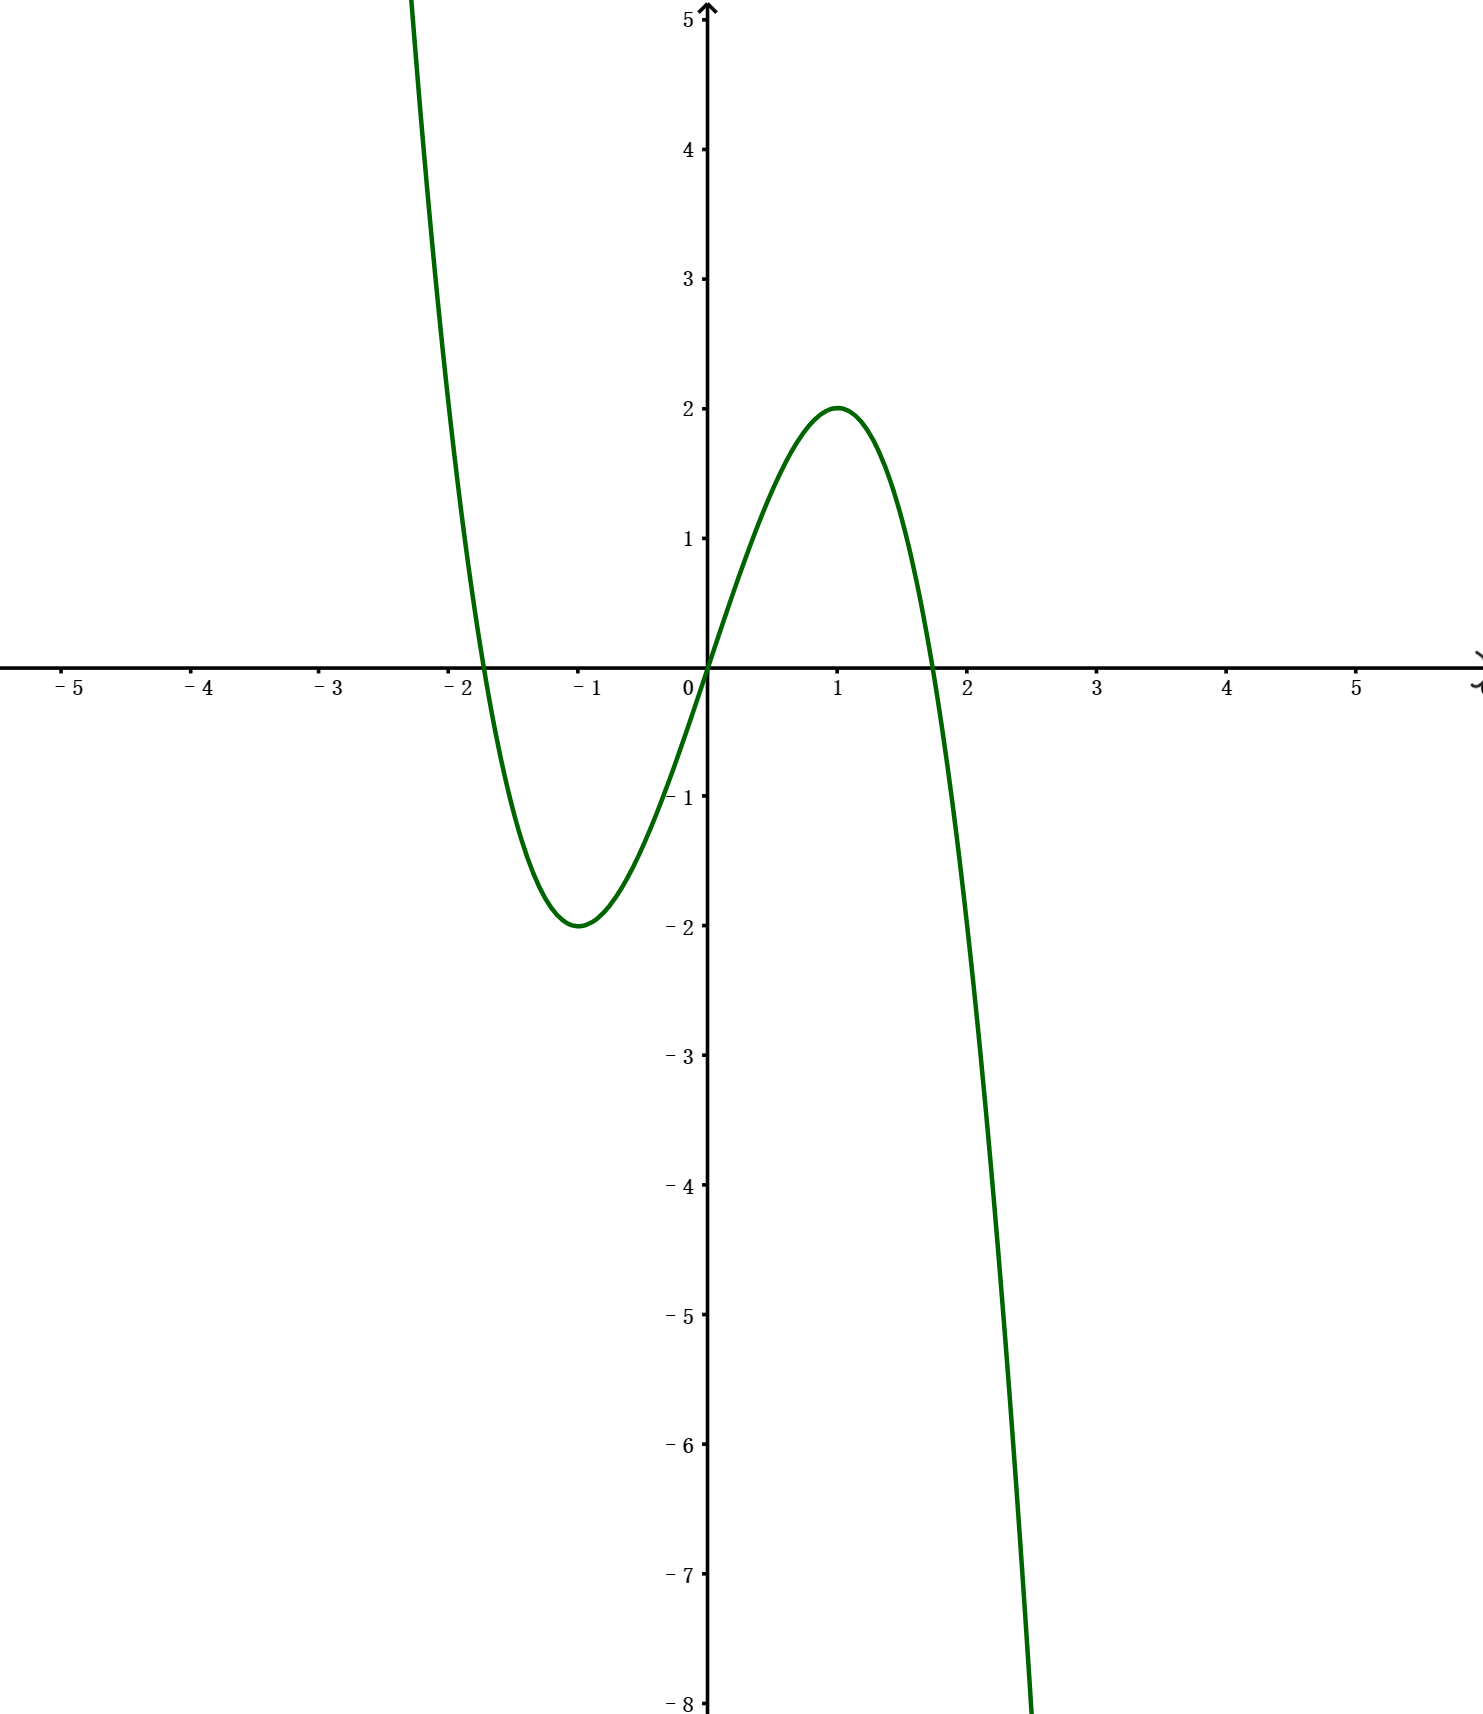
\includegraphics{pictureone.png}
		\caption{$f(x)=3x-x^{3}$}
	\end{figure}
	\chapter{最值问题}
	\textbf{闭区间上的最值问题}
	
	$f(x)$在闭区间$[a,b]$上连续可导,$f(x)$在$[a,b]$上一定存在最大值$M$和最小值$m$.其中$M=Max \left\lbrace f(a),f(b),f(x_{0})\right\rbrace $,\ $m=Min \left\lbrace f(a),f(b),f(x_{0})\right\rbrace $,$f(x_{0})$是函数的极值.
	
	我们来看一个简单的例子:$f(x)=\frac{x}{\ln x},x\in [2,e^{3}]$
	
	我们对$f(x)$求导,得到$f^{'}(x)=\frac{\ln x-1}{(\ln x)^{2}}$,令$f^{'}(x)=0$得到$x=e$是函数的驻点.
	
	当$x\in (2,e),f^{'}(x)<0$,$f(x)$单调递减;当$x\in (e,e^{2}),f^{'}(x)>0$,$f(x)$单调递增.\ $f(e)=e,f(2)=\frac{2}{\ln 2},f(e^{2}=\frac{e^{2}}{2})$,$f(x)$在区间$[2,e^{2}]$上的最大值$M= Max\left\lbrace f(2),f(e),f(e^{2})\right\rbrace \ \rightarrow M=\frac{e^{2}}{2}$;$f(x)$在区间$[2,e^{2}]$上的最小值$m= Min\left\lbrace f(2),f(e),f(e^{2})\right\rbrace \ \rightarrow m=e$.
	
	当然生活中我们还能够碰到其他的问题,比如:
	
	(1).已知一条绳子长为$l$,将它围成两个正方形,正方形面积之和的最大值?
	
	我们不妨设其中一个正方形的边长为$x$,另一个正方形的边长为$\frac{l-4x}{4}$,两个正方形面积$S=x^{2}+(\frac{l}{4}-x)^{2}$.
	
	$S^{'}=2x-2(\frac{l}{4}-x)$,令$S^{'}=0$,得到函数的驻点$x=\frac{l}{8}$,$S$在闭区间$[0,\frac{l}{4}]$上的最大值$M$和最小值$m$满足:$M=Max\left\lbrace S(0),S(\frac{l}{8}),S(\frac{l}{4})\right\rbrace;\ m=Min\left\lbrace S(0),S(\frac{l}{8}),S(\frac{l}{4})\right\rbrace $.
	
	$S(0)=\frac{l^{2}}{16},S(\frac{l}{8})=\frac{l^{2}}{32},S(\frac{l}{4})=\frac{l^{2}}{16}$.因此$M=\frac{l^{2}}{16},m=\frac{l^{2}}{32}$
	
	(2).一个长方体体积固定为$V$,底面为正方形,无盖,这个无盖长方体表面积$S_{max}$?
	
	我们不妨设底边边长为$x$,高为$h=\frac{V}{x^{2}}$,$S=x^{2}+\frac{4V}{x}$.
	
	对$S$求导得到$S^{'}=2x-\frac{4V}{x^{2}}$,令$S^{'}=0$,得到$x=(2V)^{\frac{1}{3}}$,此时$h=2^{-\frac{2}{3}}V^{\frac{1}{3}}$.
	
	$S_{max}=2^{\frac{2}{3}}V^{\frac{2}{3}}+2^{\frac{5}{3}}V^{\frac{2}{3}}$,此时$\frac{x}{h}=2$.
	
	我们也可以使用隐函数求导的方式来解决这个问题,我们有以下的两个式子:
	$$\left\{\begin{array}{c}
		S=x^{2}+4xh\\V=x^{2}h
	\end{array}\right.$$
	对上面的两个式子求导得到:$\left\{\begin{array}{c}
		\frac{\mathrm{d}S}{\mathrm{d}x}=2x+4h+4xh^{'}\\0=2xh+x^{2}h^{'}
	\end{array}\right.\Rightarrow \frac{\mathrm{d}S}{\mathrm{d}x}=2x-4h$.
	
	我们令$\frac{\mathrm{d}S}{\mathrm{d}x}=0$得到当$\frac{x}{h}=2$时,$S_{max}.$
	\chapter{相关变率}
	我们以几个具体的例子来说明这一节的问题:
	
	1.已知警察局在$B$点,测速点在$A$点,汽车从$C$向$A$行驶,满足$AB=30km$,汽车相对于警察局的速度为$80km/h$,求测速点在距离汽车$x_{0}$处测得汽车的速度.
	\begin{figure}[htbp]
		\centering
		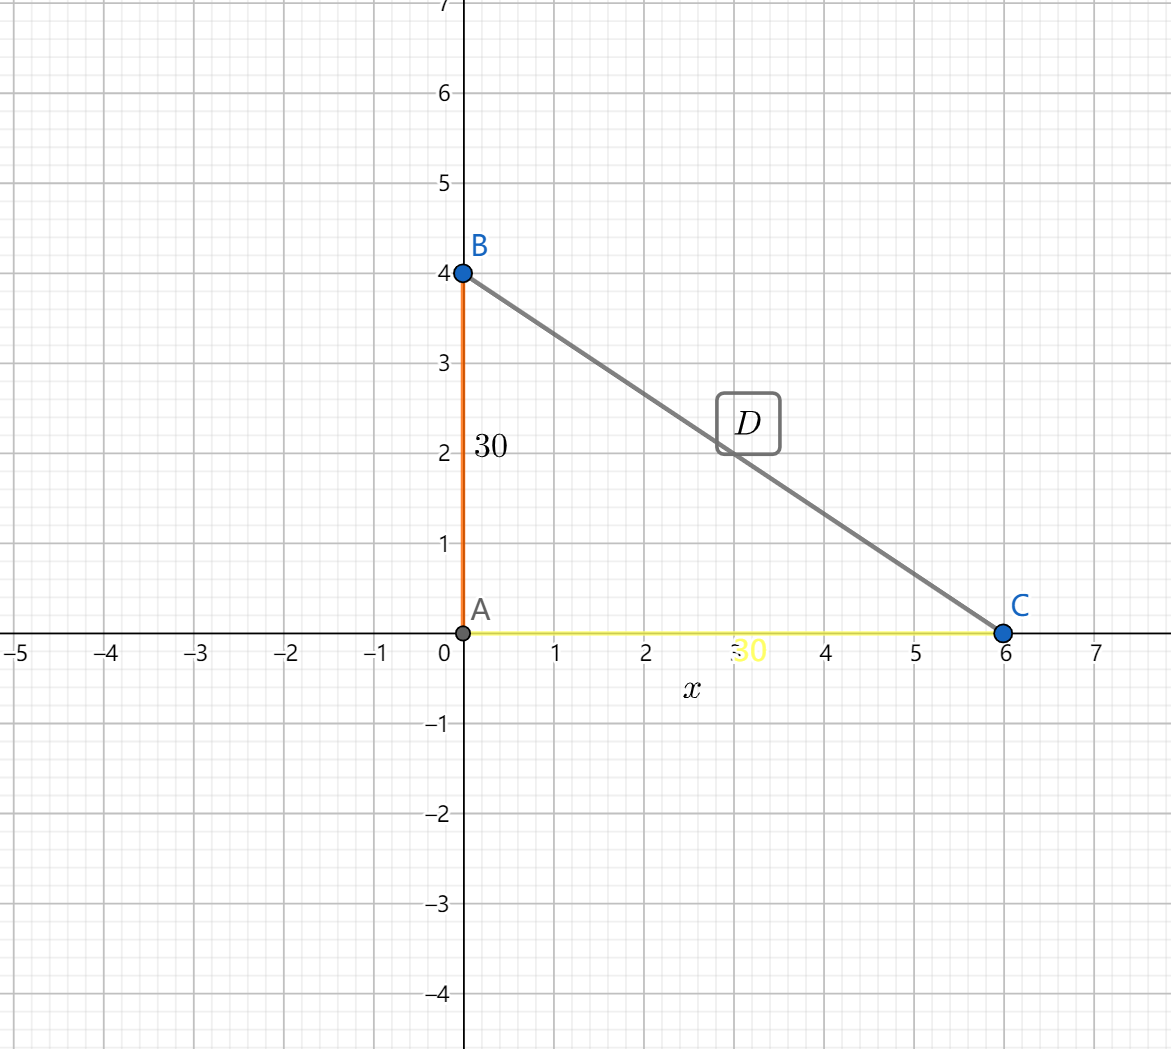
\includegraphics[width=0.5\textwidth]{picturetwo.png}
		\caption{警察问题图}
	\end{figure}

	我们由题意得到:$\left\{\begin{array}{c}
		D=30^{2}+x^{2}\\\frac{\mathrm{d}D}{\mathrm{d}t}=80
	\end{array}\right.\Rightarrow \left\{\begin{array}{c}
	\frac{\mathrm{d}D}{\mathrm{d}t}=2x\frac{\mathrm{d}x}{\mathrm{d}t}\\\frac{\mathrm{d}D}{\mathrm{d}t}=80
	\end{array}\right.$
	我们得到:
	$$\frac{\mathrm{d}x}{\mathrm{d}t}=\frac{40}{x}\Rightarrow \frac{\mathrm{d}x_{0}}{\mathrm{d}t}=\frac{40}{x_{0}}$$

	2.已知$A(0,0),B(a,b)$,有一绳子长$l>|AB|$,将绳子固定在$A,B$两点,拉紧绳子,绳子上的$D$点运动轨迹如下图$(10.2)$.
	\begin{figure}[htbp]
		\centering
		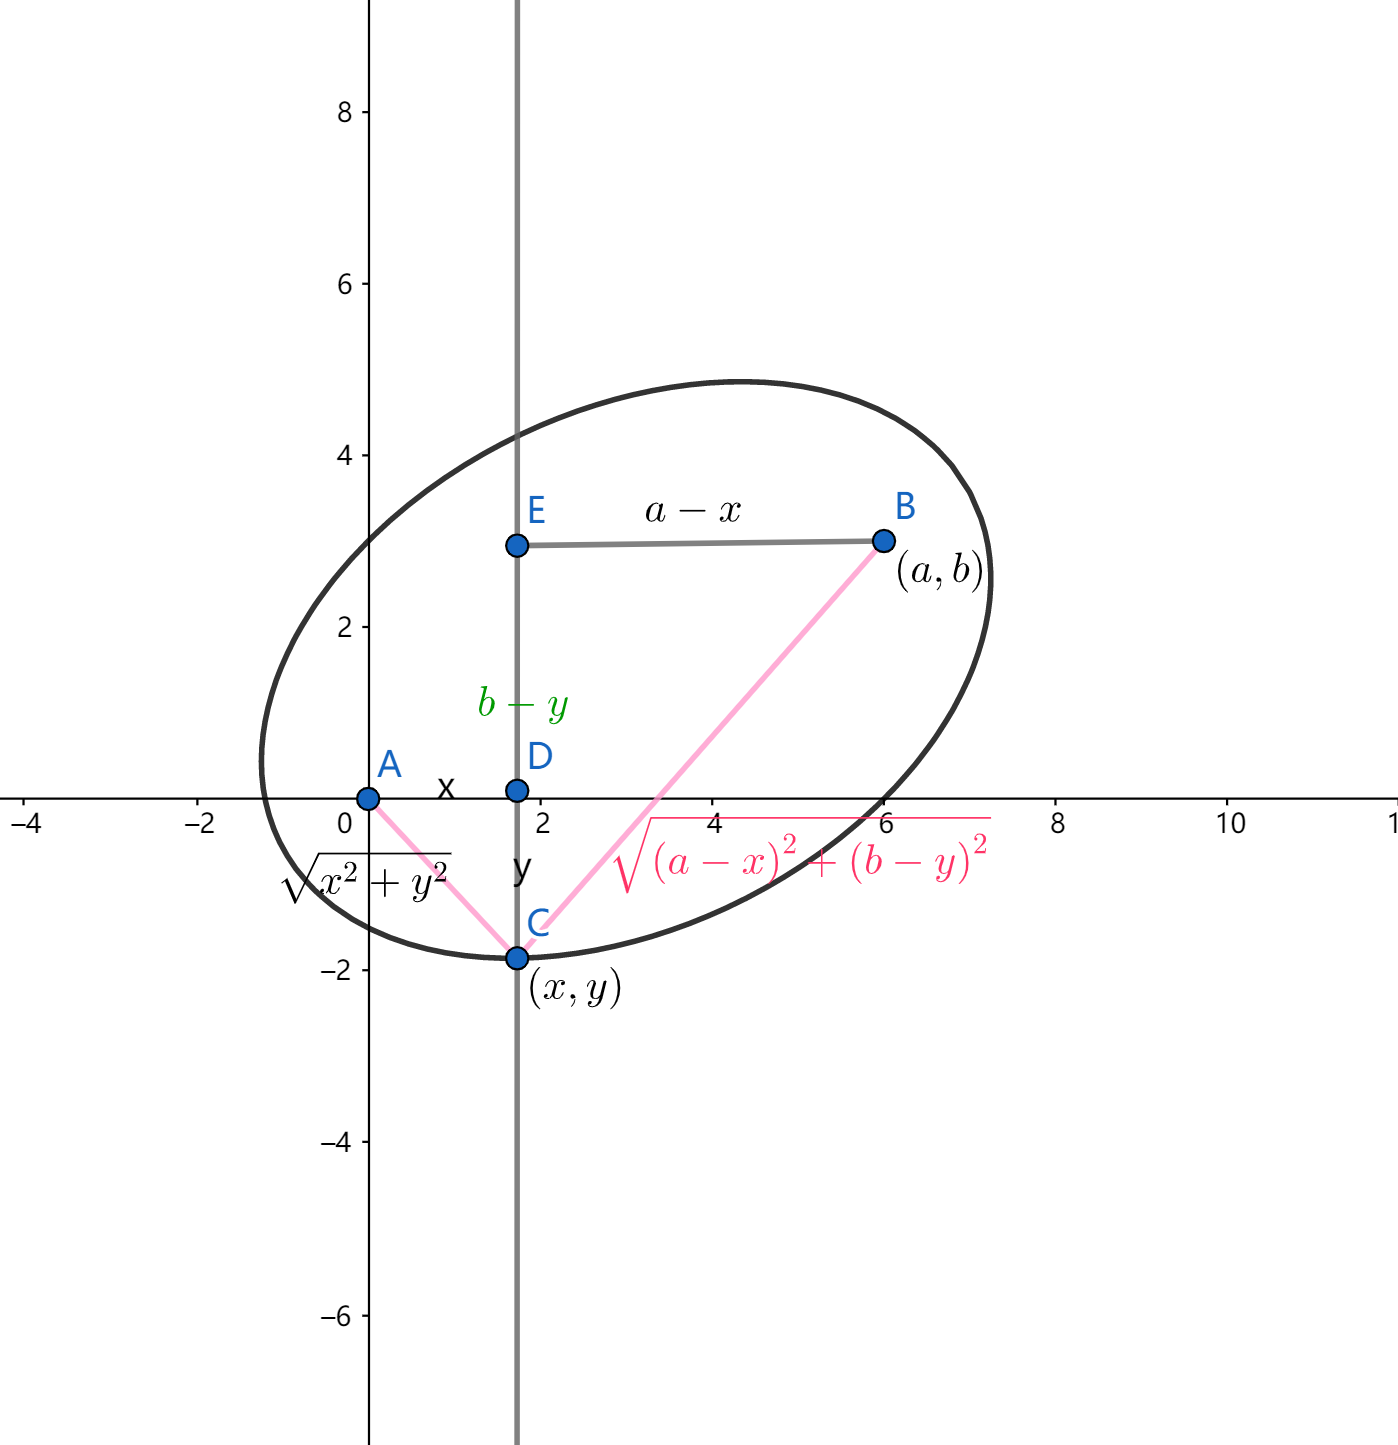
\includegraphics[width=0.5\textwidth]{picturethree.png}
		\caption{绳子问题图}
	\end{figure}
	设$D$点坐标为$(x,y)$,我们可以得到$|AC|+|BC|=l$,也就是$\sqrt{x^{2}+y^{2}}+\sqrt{(a-x)^{2}+(b-y)^{2}}=l$.我们发现$y_{D}$最小值在$y^{'}=0$时取到;这时候我们有$\angle ACD=\angle BCE$,这也是椭圆的几何性质.
	\chapter{牛顿迭代法及应用}
	我们通过一个例子来看一下牛顿迭代法,比如求解方程$f(x)=0$
	
	不妨设$x=r$是方程的解,我们选择$x=x_{0}$作为$r$的初始近似值,过点$(x_{0},f(x_{0}))$做曲线$f(x)$的切线$L_{0}$,$L_{0}:y=f(x_{0})+f^{'}(x_{0})(x-x_{0})$,$L$与$x$轴交点横坐标$x_{1}=x_{0}-\frac{f(x_{0})}{f^{'}(x_{0})}$,则称$x_{1}$是$r$的一次近似值,过点$(x_{1},f(x_{1}))$做曲线$f(x)$的切线$L_{1}$,$L_{1}:y=f(x_{1})+f^{'}(x_{1})(x-x_{1})$,$L_{1}$与$x$轴交点横坐标$x_{2}=x_{1}-\frac{f(x_{1})}{f^{'}(x_{1})}$,则称$x_{2}$是$r$的二次近似值,不断重复这个过程,我们得到$r$的近似值序列,$x_{n+1}=x_{n}+\frac{f(x_{n})}{f^{'}(x_{n})}$,以上被称为牛顿迭代公式.
	
	当然,牛顿迭代法并不适用于所有的情况,我们必须要求:
	
	1.$x_{0}$选取在$r$附近.
	
	2.二阶导数不是特别大,一阶导数不接近0.
	
	我们用公式来表示的话就是:$f(x)=0$的解为$x=r$,取位于$x=r$附近的$x=x_{0}$进行迭代,我们有:
	\begin{equation}
		\left\{\begin{array}{c}
			x_{1}=x_{0}-\frac{f(x_{0})}{f^{'}(x_{0})}\\	x_{2}=x_{1}-\frac{f(x_{1})}{f^{'}(x_{1})}\\......\\	x_{n+1}=x_{n}-\frac{f(x_{n})}{f^{'}(x_{n})}
		\end{array}\right.
	\end{equation}
	\chapter{中值定理及重要不等式}
	\textbf{中值定理}
	
	\textbf{注}:中值定理又被称为微分中值定理和拉格朗日中值定理.
	
	$f(x)$在区间$(a,b)$上可导,$f(x)$在区间$[a,b]$上连续,那么$\exists\ c\in (a,b)$满足$f^{'}(c)=\frac{f(b)-f(a)}{b-a}\Leftrightarrow $$\exists\ c\in (a,b)$满足$f(b)=f(a)+f^{'}(c)(b-a)$.
	
	\hspace{\fill}\
	
	特别的,当$f(a)=f(b)$时,我们得到\textbf{罗尔定律}:$f(x)$在区间$(a,b)$上可导,$f(a),f(b)$存在且相等,那么$\exists\ c\in (a,b)$满足$f^{'}(c)=0$.
	
	
	\begin{proof}
		\hspace{\fill}\
		我们首先来证明罗尔定理,$f(x)$在闭区间$[a,b]$上连续,$f(x)$在闭区间$[a,b]$上一定存在最大值和最小值,且$f(a)=f(b)$,所以$\exists\ c\in [a,b]$,使得$f(c)$是最大值或者最小值.我们不妨假设$f(c)$是最大值,因此我们有以下的式子:
		$$\left\{\begin{array}{c}
			\lim\limits_{x\rightarrow c^{+}}\frac{f(x)-f(c)}{x-c}\le 0\\\lim\limits_{x\rightarrow c^{-}}\frac{f(x)-f(c)}{x-c}\geq 0
		\end{array}\right.$$
		$f(x)$在$[a,b]$上连续,$\lim\limits_{x\rightarrow c^{+}}\frac{f(x)-f(c)}{x-c}=\lim\limits_{x\rightarrow c^{-}}\frac{f(x)-f(c)}{x-c}$,因此$\lim\limits_{x\rightarrow c}\frac{f(x)-f(c)}{x-c}=f^{'}(c)=0$得证.
		
		接下来我们继续来证明中值定理,我们构造$g(x)=f(a)+\frac{f(b)-f(a)}{b-a}(x-a)$,令$G(x)=f(x)-g(x)$,我们有$G(a)=G(b)=0$,$f(x),g(x)$在区间$[a,b]$上连续,利用罗尔定律,我们知道$\exists\ c\in [a,b]$使得$G^{'}(c)=0$.我们还可以得到下面的两种形式:
		$$\frac{f(b)-f(a)}{b-a}=f^{'}(\varepsilon)\ \Leftrightarrow f(b)=f(a)+f^{'}(\varepsilon)(b-a),\ \varepsilon \in \ (a,b)$$
	\end{proof}
	\textbf{重要不等式}
	
	$e^{x}>1+x+\frac{x^{2}}{2}+\frac{x^{3}}{6}+...+\frac{x^{n}}{n!}\Leftrightarrow \ e^{x}>\sum_{k=0}^{n}\frac{x^{k}}{k!},\ x\in (0,+\infty)$
	
	我们采用数学归纳法来证明这个不等式:
	
	(1).当$n=1$时,$e^{x}>1+x$.
	
	(2).假设当$n=r$时不等式$e^{x}>1+x+\frac{x^{2}}{2}+\frac{x^{3}}{6}+...+\frac{x^{r}}{r!}$成立,当$n=r+1$时,令$f(x)=e^{x}-1+x+\frac{x^{2}}{2}+\frac{x^{3}}{6}+...+\frac{x^{r}}{r!}+\frac{x^{r+1}}{(r+1)!}$,$f(0)=0$,$f^{'}(x)=e^{x}-1+x+\frac{x^{2}}{2}+\frac{x^{3}}{6}+...+\frac{x^{r}}{r!}>0$,因此$f(x)$单调递增,$f(x)>f(0)\Rightarrow f(x)>0$,得证.
	\chapter{无穷小量和不定积分}
	\textbf{微分}
	
	对于$y=f(x)$,我们有$\mathrm{d}y=f^{'}(x)\mathrm{d}x$,其中$\mathrm{d}y$为$y$的微分,也被称作为$f$的微分;我们将上面的式子稍作变形得到$\frac{\mathrm{d}y}{\mathrm{d}x}=f^{'}(x)$,这说明函数在某一点处可微和在某一点处可导是完全等价的,同时我们观察导函数的表达式可以得到,导函数是由两个无穷小量相比得到.
	
	\textbf{不定积分}
	
	$G(x)=\int g(x)\mathrm{d}x$,\ $G(x)$是$g(x)$的反导数,也被称作为$g(x)$的不定积分.
	
	积分唯一性:假设$F^{'}=G^{'}$,我们有$F(x)=G(x)+C$.
	
	\textbf{常见的不定积分公式}
	\begin{equation}
		\left\{\begin{array}{c}
		\int x^{a}\mathrm{d}x=\frac{x^{a+1}}{a+1}+C,\ a\neq 1\\\\\int \sin x\mathrm{d}x=-\cos x+C\\\int cos  x\mathrm{d}x=\sin x+C\\\int \sec^{2}x\mathrm{d}x=\tan x+C\\\\\int \frac{1}{x}\mathrm{d}x=\ln|x|+C\\\int e^{x}\mathrm{d}x=e^{x}+C\\\\\int \frac{1}{\sqrt{1-x^{2}}}\mathrm{d}x=\arcsin x+C\\\int \frac{1}{1+x^{2}}\mathrm{d}x=\tan x+C
	\end{array}\right.
	\end{equation}

	\textbf{换元法求不定积分}
	
	(1).$\int x^{3}(x^{4}+2)^{5}\mathrm{d}x$
	
	(2).$\int \frac{x\mathrm{d}x}{\sqrt{1+x^[2]}}$
	
	(3).$\int xe^{-x^{2}}$
	
	(4).$\int \sin x\cos x\mathrm{d}x$
	
	(5).$\int\frac{\mathrm{d}x}{x\ln x}$
	
	\chapter{微分方程和分离变量}
	\textbf{微分方程}
	
	我们以一个具体的方程来说:$(\frac{\mathrm{d}}{\mathrm{d}x}+x)y=0$
	这个式子可以化为$$\frac{\mathrm{d}y}{\mathrm{d}x}=-xy\Leftrightarrow \frac{\mathrm{d}y}{y}=-x\mathrm{d}x$$
	对上式两边同时求不定积分得到:$$\int \frac{1}{y}\mathrm{d}y=\int -x\mathrm{d}x\Leftrightarrow \ln |y|=-\frac{1}{2}x^{2}+C$$
	因此这个微分方程的解为$y=\pm Ae^{-\frac{1}{2}x^{2}},A=e^{C}$(正态分布)
	
	我们会碰到这样一类的微分方程:$\frac{\mathrm{d}y}{\mathrm{d}x}=f(x)g(y)$,我们知道这和我们之前隐函数求导的结果很相似,我们解出这个方程需要分离变量:
	$$\frac{1}{g(y)}\mathrm{d}y=f(x)\mathrm{d}x\Leftrightarrow \int \frac{1}{g(y)}\mathrm{d}y=\int f(x)\mathrm{d}x$$
	我们不妨设$H(y)=\frac{1}{g(y)}\mathrm{d}y,F(x)=\int f(x)\mathrm{d}x$,我们有:$$H(y)-F(x)=C\Leftrightarrow y=H^{-1}(F(x)+C)$$
	我们来看下一个例子:$\frac{\mathrm{d}y}{\mathrm{d}x}=2\frac{y}{x}$.
	
	我们利用分离变量的方法得到:$H(y)=\ln |y|,F(x)=\ln |x|^{2}$,因此$y=Ax^{2}$,经过论证和讨论$A\in \ R$,但是我们发现函数在$x=0$处没有定义,因此$x<0$和$x>0$两部分的$A$可以不相同.
	
	\chapter{定积分}
	\textbf{曲边梯形的面积}
	
	$f(x)$在$[a,b]$上连续,求$f(x)$和$x=a,x=b$以及$x$轴围成的曲边梯形面积$S$.
	$$S=\int_{a}^{b}f(x)\mathrm{d}x$$
	
	我们以具体的例子来说明,$f(x)=x^{2}$与$x=0,x=b,y=0$围成的图形的面积.
	我们将$[0,b]$分为$n$份,将图形面积近似处理为$n$个长方形的面积之和:
	$$S\approx\sum_{i=1}^{n}f(x_{i})\frac{b}{n}\Rightarrow S=\lim\limits_{n\rightarrow +\infty}\sum_{i=1}^{n}f(x_{i})\frac{b}{n}$$
	我们将$\sum_{i=1}^{n}f(x_{i})\frac{b}{n}$称为黎曼和,而黎曼和的极限就是黎曼积分或者称之为定积分.
	\chapter{微积分第一基本定理}
	如果$F(x)=f^{'}(x)$,那么我们有$\int_{a}^{b} f^{'}(x)\mathrm{d}x=F(b)-F(a)$,也可以写作$\int_{a}^{b} f^{'}(x)\mathrm{d}x=F(x)|_{x=a}^{x=b}$,这就是微积分第一基本定理.
	
	我们来看上一节定积分中的几个例子:
	
	(1).$\int_{a}^{b}x^{2}\mathrm{d}x=\frac{x^{3}}{3}|_{x=a}^{x=b}$
	
	(2).$\int_{0}^{\pi}\sin x\mathrm{d}x=(-\cos x)|_{x=0}^{x=\pi}=2$
	
	\textbf{定积分运算法则}
	
	1.$\int_{a}^{b}(f(x)+g(x))\mathrm{d}x=\int_{a}^{b}f(x)\mathrm{d}x+\int_{a}^{b}g(x)\mathrm{d}x$
	
	\hspace{\fill}\
	
	2.$\int_{a}^{b}Cf(x)\mathrm{d}x=C\int_{a}^{b}f(x)\mathrm{d}x$
	
	\hspace{\fill}\
	
	3.$\int_{a}^{b}f(x)\mathrm{d}x=\int_{a}^{c}f(x)\mathrm{d}x+\int_{c}^{b}f(x)\mathrm{d}x$
	
	\hspace{\fill}\
	
	4.$\int_{a}^{b}f(x)\mathrm{d}x=-\int_{b}^{a}f(x)\mathrm{d}x$
	
	\hspace{\fill}\
	
	5.如果$f(x)\leq g(x)$,我们有$\int_{a}^{b}f(x)\mathrm{d}x\leq \int_{a}^{b}g(x)\mathrm{d}x,\ (a<b)$
	
	\hspace{\fill}\
	
	6.$\int_{u_{1}}^{u_{2}}g(u)\mathrm{d}u=\int_{x_{1}}^{x_{2}}g(u)u^{'}(x)\mathrm{d}x$
	
	\hspace{\fill}\
	
	7.如果$f(x)$是奇函数,$\int_{-a}^{a}f(x)\mathrm{d}x=0$;如果$f(x)$是偶函数,$\int_{-a}^{a}f(x)\mathrm{d}x=2\int_{0}^{a}f(x)\mathrm{d}x$
	\chapter{微积分第二基本定理}
	假设$G(x)=\int_{a}^{x}f(t)\mathrm{d}t$,我们有$G^{'}(x)=f(x)$,这就是微积分第二定理.
	\begin{proof}
		我们根据黎曼和的定义:$\int_{0}^{x} f(x)=\lim\limits_{n\rightarrow +\infty}\sum_{i=1}^{n}f(x_{i})(\frac{x}{n})$
		
		$$G^{'}(x)=\lim\limits_{\Delta x\rightarrow 0}\frac{G(x+\Delta x)-G(x)}{\Delta x}$$
		$$G(x)=\lim\limits_{n\rightarrow +\infty}\sum_{i=1}^{n}f(x_{i})(\frac{x}{n})$$
		$$G(x+\Delta x)=\lim\limits_{n\rightarrow +\infty}\sum_{i=1}^{n}f(x_{i})(\frac{x}{n})+f(x)\Delta x$$
		因此:$G^{'}(x)=f(x)$
	\end{proof}

	\hspace{\fill}\

	1.$F(x)=\int_{1}^{x}\frac{1}{t}\mathrm{d}t$
	
	我们有$F^{'}(x)=\frac{1}{x},F^{''}(x)=-\frac{1}{x^{2}},F(1)=\int_{1}^{1}\frac{1}{t}\mathrm{d}t=0,F^{'}(1)=1$.
	
	函数$F(x)$有许多值得我们注意的性质:
	
	(1).当$x\in \left(0,1 \right),F(x)<0$;当$x\in \left(1,+\infty \right),F(x)>0$.
	
	(2).$F(ab)=F(a)+F(b)$
	
	(3).$F(x)=-F(\frac{1}{x})$
	
	\hspace{\fill}\
	
	2.$G(x)=\int_{0}^{x}e^{-t^{2}}\mathrm{d}t$
	
	我们有$\left\lbrace \begin{array}{c}
		G^{'}(x)=e^{-x^{2}}\\
		G^{''}(x)=-2xe^{-x^{2}}\\
		G(0)=\int_{0}^{0}e^{-t^{2}}\mathrm{d}t=0\\
		G^{'}(0)=1\\G^{''}(0)=-2
	\end{array}\right. $

	我们同样可以得到这个函数的一些性质:
	
	(1).G(-x)=-G(x)
	
	(2).当$x\in \left( -\infty,0\right),G^{'}(x)<0$;当$x\in \left( 0,+\infty\right),G^{'}(x)>0$.
	
	(3).当$x\rightarrow -\infty,G(x)\rightarrow -\frac{\sqrt{\pi}}{2}$;当$x\rightarrow +\infty,G(x)\rightarrow \frac{\sqrt{\pi}}{2}$
	
	\hspace{\fill}\
	
	3.我们在第二个函数基础上进行改变,$R(x)=\frac{2}{\sqrt{\pi}}G(x)$,这是正态分布的函数.
	
	\hspace{\fill}\
	
	4.$\left\lbrace \begin{array}{c}
	C(x)=\int_{0}^{x}\cos(t^{2})\mathrm{d}t\\ S(x)=\int_{0}^{x}\sin(t^{2})\mathrm{d}t\\ H(x)=\int_{0}^{x}\frac{\sin t}{t}\mathrm{d}t	\end{array}\right. $

	\hspace{\fill}\
	
	5.$L(x)=\int_{2}^{x}\frac{\mathrm{d}t}{\ln t}$,这个函数表示的是小于$x$的素数的个数.即$L(x)=(N(primes)<x)$(黎曼假设)
	\chapter{定积分在对数和几何上的应用}
	\textbf{曲线围成的面积}
	
	函数$f(x),g(x)$在区间$[a,b]$中围成的面积$S$,求$S$表达式.
	$$S=\int_{a}^{b}|f(x)-g(x)|\mathrm{d}x$$
	我们来看一个例子:曲线$x=y^{2}$和$y=x-2$围成的面积
	
	我们知道:$S=\int_{0}^{1}2\sqrt{x}\mathrm{d}x+\int_{1}^{4}(\sqrt{x}-x+2)\mathrm{d}x=\frac{9}{2}$
	
	当然我们还可以换一种思维:$S=\int_{-1}^{2}(y+2-y^{2})\mathrm{d}y=\frac{9}{2}$
	\chapter{壳层法、圆盘法求体积}
	1.\textbf{圆盘法求旋转体体积}
	
	已知函数$f(x)$在$[a,b]$上连续,且$f(x)>0,x\in \ [a,b]$,将$f(x)$绕$x$轴旋转一周得到的旋转体体积$V$.
	
	我们由微分得:$\mathrm{d}V=\pi y^{2}\mathrm{d}x$,我们对这个式子积分得到:
	$$V=\int_{a}^{b}\pi (f(x))^{2}\mathrm{d}x$$
	我们可以依照这个推导出球的体积公式,假设$f(x)=\sqrt{a^{2}-x^{2}},x\in \ [-a,a]$,将$f(x)$绕$x$轴旋转一周得到一个半径为$r=a$的球.
	$$V=\int_{-a}^{a}\pi (f(x))^{2}\mathrm{d}x\Rightarrow V=\pi \int_{-a}^{a}(a^{2}-x^{2})\mathrm{d}x=\frac{4a^{3}}{3}\pi$$
	
	2.\textbf{壳层法求}
	
	我们需要一个具体的例子来说明这个方法,$f(x)=x^{2},x\in \ [-a.a]$,将$f(x)$绕$y$轴旋转得到的旋转体体积$V$.
	
	我们由微分得:$\mathrm{d}V=2\pi x(a^{2}-f(x))^{2}\mathrm{d}x$,对这个式子两边积分得到:
	$$V=2\pi\int_{-a}^{a}x(a^{2}-x^{2})\mathrm{d}x=\frac{a^{4}}{3}\pi$$
	\chapter{功、平均值、概率}
	1.\textbf{平均值}
	
	我们有$y=f(x),x\in\ [a,b]$,$f(x)$在$[a,b]$上连续,假设存在$a<x_{1}<x_{2}<...<x_{n}<b$,那么我们有:$$\lim\limits_{n\rightarrow +\infty}\frac{y_{1}+y_{2}+...+y_{n}}{n}=\frac{1}{b-a}\int_{a}^{b}f(x)\mathrm{d}x$$
	
	我们不难发现:$\int_{a}^{b}f(x)\mathrm{d}x=\lim\limits_{n\rightarrow 0}\sum_{i=1}^{n}f(x_{i})\frac{b-a}{n}$,这是黎曼和的形式,当$n\rightarrow +\infty$时,得到黎曼积分(定积分),我们对这个式子稍作变化得到:
	$$\frac{1}{b-a}\int_{a}^{b}f(x)\mathrm{d}x=\lim\limits_{n\rightarrow 0}\sum_{i=1}^{n}f(x_{i})\frac{1}{n}\Leftrightarrow \frac{1}{b-a}\int_{a}^{b}f(x)\mathrm{d}x=\lim\limits_{n\rightarrow 0}\frac{\sum_{i=1}^{n}f(x_{i})}{n}$$.
	我们将$\frac{1}{b-a}\int_{a}^{b}f(x)\mathrm{d}x$称作$f(x)$在$[a,b]$上的平均值.
	
	我们不妨来看几个例子:
	
	(1).$y=\sqrt{1-x^{2}}$在$[-1,1]$上的平均值.
	
	$\overline{y}=\frac{1}{2}\int_{-1}^{1}\sqrt{1-x^{2}}\mathrm{d}x=\frac{\pi}{4}$
	
	(2).$y=\sin x,x\in \ [0,\pi]$在$[0,\pi]$上的平均值.
	
	$\overline{y}=\frac{1}{\pi}\int_{0}^{\pi}\sin x\mathrm{d}x=\frac{2}{\pi}$
	
	\textbf{加权平均值}
	$$\overline{f(x)}=\frac{\int_{a}^{b}f(x)w(x)\mathrm{d}x}{\int_{a}^{b}w(x)\mathrm{d}x},\ w(x)\ is \ weight.$$
	
	\textbf{概率}
	
	假设平面内有一区域:$S\in \left\{\begin{array}{c}
		-1<x<1\\0<y<1-x^{2}
	\end{array}\right.$,从中任意取出一点,求出$P(x>\frac{1}{2})$.

	$P(x>\frac{1}{2})=\frac{\int_{\frac{1}{2}}^{1}(1-x^{2}\mathrm{d}x)}{\int_{-1}^{1}(1-x^{2})\mathrm{d}x}=\frac{5}{32}$
	
	我们继续来看一个例子:
	
	一个人在远处扔飞镖,在距离圆心$r$处单位面积被击中的次数$N=ce^{-r^{2}}$,另一个人在同心圆内,内圆半径$r_{1}$,外圆半径$r_{2}$,另一个人被飞镖击中的概率$P$.
	
	$$P=\frac{N_{part}}{N_{all}}=\frac{\int_{r_{1}}^{r_{2}}2\pi re^{-r^{2}}\mathrm{d}r}{\int_{0}^{+\infty}2\pi re^{-r^{2}}\mathrm{d}r}$$
	我们将上面的式子化简:$P=\frac{\int_{r_{1}}^{r_{2}} e^{-r^{2}}\mathrm{d}r^{2}}{\int_{0}^{+\infty}e^{-r^{2}}\mathrm{d}r^{2}}=\frac{-\int_{r_{1}^{2}}^{r_{2}^{2}}e^{-t}\mathrm{d}t}{-\int_{0}^{+\infty}e^{-t}\mathrm{d}t}=e^{-r_{1}^{2}}-e^{-r_{2}^{2}}$
	\chapter{数值积分}
	$y=f(x)$在$[a,b]$上连续,在$(a,b)$上可导.
	
	1.\textbf{黎曼和}
	
	假设存在$a=x_{0}<x_{1}<x_{2}<...<x_{n-1}<x_{n}=b$,满足$\Delta x=x_{i}-x_{i-1}$,我们有$y_{0}=f(x_{0}),y_{1}=f(x_{1}),...y_{n}=f(x_{n})$.我们可以得到函数的左右黎曼和:
	$$\left\{\begin{array}{c}
		(y_{0}+y_{1}+...+y_{n-1})\Delta x \qquad Left\\(y_{1}+y_{2}+...+y_{n})\Delta x \qquad Right
	\end{array}\right.$$

	2.\textbf{曲边梯形法}
	
	和黎曼和类似,不过是采用梯形的面积和近似于曲边梯形面积,而不是矩形.
	
	$$S=\Delta x(\frac{y_{0}}{2}+y_{1}+y_{2}+...+\frac{y_{n}}{2})=\frac{Left+Right}{2}$$
	
	3.\textbf{辛普森方法}
	
	采用一种加权求和的方式,将曲边梯形分成$n$个曲边梯形,$n$是偶数,我们有下面的式子:
	$$\left\{\begin{array}{c}
		S_{1}=\Delta x(\frac{y_{0}+4y_{1}+y_{2}}{6})\\S_{2}=\Delta x(\frac{y_{0}+4y_{1}+y_{2}}{6})\\......\\S_{n}=\Delta x(\frac{y_{n-2}+4y_{n-1}+y_{n}}{6})
	\end{array}\right.$$
	$$S=\Delta x(y_{0}+4y_{1}+2y_{2}+4y_{3}+2y_{4}+...+y_{n})$$
	
	我们来具体看一个例子,就可以明白三种方法的优劣性:
	$a=\int_{1}^{2}\frac{1}{x}\mathrm{d}x$
	
	不妨令$n=2$;
	
	1.在梯形法中,$S=\frac{1}{2}(\frac{1}{2}+\frac{2}{3}+\frac{1}{2})=\frac{17}{24}\approx 0.7083$
	
	2.在辛普森法中,$S=\frac{1}{6}(1+\frac{8}{3}+\frac{1}{4})=\frac{25}{36}\approx0.69444$
	
	我们知道:$\ln 2\approx 0.69314$,辛普森法的误差$\Delta y\approx 0.0013$
	
	\textbf{重要积分}
	
	我们接下来看一个很重要的积分:$V=\int_{0}^{+\infty}2\pi re^{-r^{2}}\mathrm{d}x=\pi$
	
	我们可以将$V$看作是一个旋转体的体积,是将$G(x)=e^{-x^{2}}$绕$y$轴旋转一周得到,此时的$y$轴变成$z$轴,旋转体上任一点$A$满足$z_{A}=e^{-r^{2}}$,其中$r$是距离原点的距离.我们将这个旋转体沿$y$轴切片$$V=\int_{-\infty}^{+\infty}A(y)\mathrm{d}y$$
	我们关键是要求出$A(y)$的表达式,$$A(y)=\int_{-\infty}^{+\infty}e^{-x^{2}-y^{2}}\mathrm{d}x=e^{-y^{2}}\int_{-\infty}^{+\infty}e^{-x^{2}}\mathrm{d}x$$
	我们不妨令$Q=\int_{-\infty}^{+\infty}e^{-x^{2}}\mathrm{d}x$,那么我们发现:
	$$V=Q\int_{-\infty}^{+\infty}e^{-y^{2}}\mathrm{d}y=Q^{2}$$
	
	对于$F(x)=\int_{0}^{x}e^{-t^{2}}\mathrm{d}t$,我们发现$F(+\infty)=\frac{Q}{2}$,所以$V=4(F(+\infty))^{2}\Rightarrow F(+\infty)=\frac{\sqrt{\pi}}{2}$
	\chapter{三角函数的积分和三角替换}
	如下图所示,对角线上的三角函数乘积为1,三个倒三角满足上面两个顶点平方和等于下面顶点的平方和.
	\begin{figure}[htbp]
		\centering
		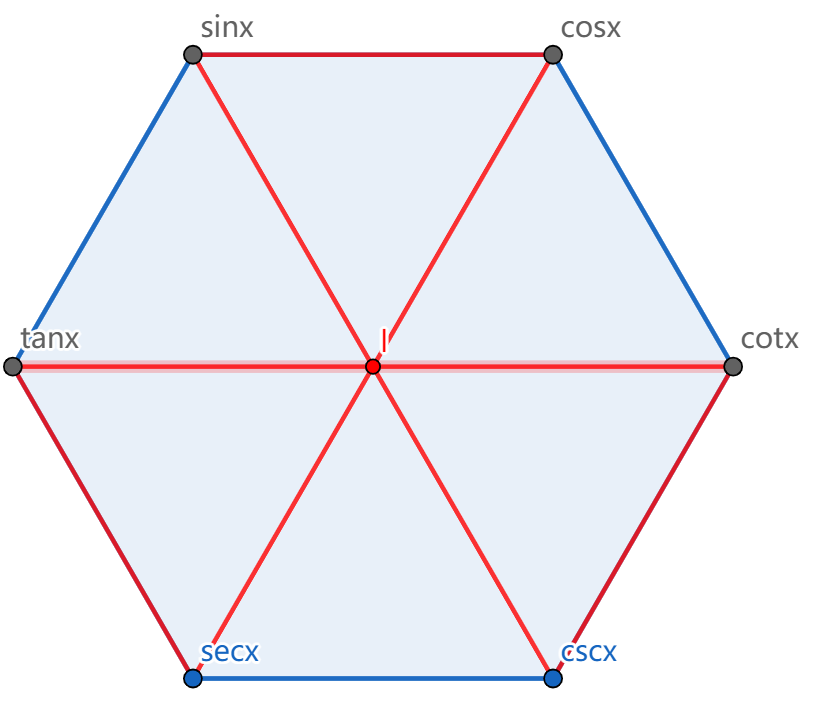
\includegraphics[width=0.4\textwidth]{picturefour.png}
		\caption{六个三角函数关系图}
	\end{figure}
	$$\left\{\begin{array}{c}
		\sec x=\frac{1}{\cos x}\\\csc x=\frac{1}{\sin x}\\\cot x=\frac{1}{tan x}\\\sin^{2}x+\cos^{2}x=1\\tan^{2}x+1=sec^{2}x\quad (Important)\\1+cot^{2}=csc^{2}x
	\end{array}\right.$$

	\textbf{三角恒等式和三角变换}
	$$\left\{\begin{array}{c}
		\sin^{2} \theta+\cos^{2} \theta=1\\\sin 2\theta=2\sin \theta\cos \theta\\\cos 2\theta=1-2\sin^{2}\theta=2\cos^{2}\theta -1\\\sin (\alpha\pm \beta)=\sin \alpha\cos \beta\pm \cos \alpha\sin\beta\\\cos (\alpha\pm \beta)=\cos \alpha\cos \beta\mp \sin \alpha\sin\beta
	\end{array}\right.$$
	
	\textbf{和差化积、积化和差公式}
	$$\left\{\begin{array}{c}
		\sin (\alpha+\beta)+\sin (\alpha-\beta)=2\sin \alpha\cos\beta\\\sin (\alpha+\beta)-\sin (\alpha-\beta)=2\cos \alpha\sin\beta\\\cos (\alpha+\beta)+\cos (\alpha-\beta)=2\cos \alpha\cos\beta\\\cos (\alpha+\beta)-\cos (\alpha-\beta)=-2\sin \alpha\sin\beta\\\\\sin\alpha+\sin\beta=2\sin\frac{\alpha+\beta}{2}\cos\frac{\alpha-\beta}{2}\\\cos\alpha+\cos\beta=2\cos\frac{\alpha+\beta}{2}\cos\frac{\alpha-\beta}{2}\\\sin\alpha-\sin\beta=2\cos\frac{\alpha+\beta}{2}\sin\frac{\alpha-\beta}{2}\\\cos\alpha-\cos\beta=-2\cos\frac{\alpha+\beta}{2}\cos\frac{\alpha-\beta}{2}
	\end{array}\right.$$

	1.我们来看一个例子:$\ \int \sin^{n}(x)\cos^{m}(x)\mathrm{d}x;\ m,n=0,1,2...$
	
	(1).当$m,n$至少有一个是奇数的时候,我们不妨假设$m$是奇数,原不定积分可以化为下面的形式:$$\int \sin^{n}(x)cos^{m-1}\mathrm{d}\sin x\Rightarrow \int \sin^{n}(x)(1-\sin^{2}(x))^{\frac{m-1}{2}}\mathrm{d}\sin x$$
	我们做一次三角替换$u=\sin x$,最终可以得到一个整数次幂多项式的不定积分,进而可以求解.
	
	(2).当$m,n$都是偶数的时候,需要利用倍角公式进行降幂处理,让$m,n$至少出现一个奇数.
	
	我们来看几个简单的例子:
	
	(i).$\int\sin^{2}x\cos^{2}\mathrm{d}x$
	
	(ii).$\int\cos^{2}x$
	
	\hspace{\fill}\
	
	2.我们来看三角替换的具体应用:$\int\sqrt{a^{2}-x^{2}}\mathrm{d}x$
	
	我们不妨令$x=a\sin \theta$,原不定积分可以化为:$$\int a^{2}\cos^{2}\theta\mathrm{d}\theta\Rightarrow \int a^{2}\frac{1+\cos 2\theta}{2}\mathrm{d}\theta=a^{2}(\frac{\theta}{2}+\frac{\sin 2\theta}{4})+C$$
	将$\theta=\arcsin(\frac{a}{x}),\sin2\theta=2\frac{x}{a}\sqrt{\frac{a^{2}-x^{2}}{a^{2}}}$得到:
	$$\int\sqrt{a^{2}-x^{2}}\mathrm{d}x=\frac{x\sqrt{a^{2}-x^{2}}}{2}+\frac{a^{2}}{2}\arcsin(\frac{x}{a})+C$$
	
	3.我们来求几个重要的不定积分:
	
	(1).$\int \tan x\mathrm{d}x$
	
	上面的不定积分可以化为$\int \frac{\sin x}{\cos x}\mathrm{d}x=\int -\frac{1}{\cos x}\mathrm{d}\cos x=-\ln |\cos x|+C$
	
	\hspace{\fill}\
	
	(2).$\int \cot x\mathrm{d}x$
	
	上面的不定积分可以化为$\int \frac{\cos x}{\sin x}\mathrm{d}x=\int \frac{1}{\sin x}\sin x=\ln |\sin x|+C$
	
	\hspace{\fill}\
	
	(3).$\int \frac{1}{x^{2}+a^{2}}\mathrm{d}x$
	
	原不定积分为:$\frac{1}{a}\int \frac{1}{1+(\frac{x}{a})^{2}}\mathrm{d}\frac{x}{a}=\frac{1}{a}\arctan \frac{x}{a}+C$
	
	\hspace{\fill}\
	
	(4).$\int \frac{1}{a^{2}-x^{2}}\mathrm{d}x$
	
	原不定积分可化为:$\frac{1}{2a}\int (\frac{1}{a-x}+\frac{1}{a+x})\mathrm{d}x=\frac{1}{2a}(\ln|a-x|+\ln|a+x|)+C=\frac{1}{2a}\ln|\frac{a-x}{a+x}|+C$
	
	\hspace{\fill}\
	
	(5).$\int \frac{1}{\sqrt{a^{2}-x^{2}}}\mathrm{d}x$
	
	原不定积分可以化为:$\int \frac{1}{\sqrt{1-(\frac{x}{a})^{2}}}\mathrm{d}\frac{x}{a}=\arcsin\frac{x}{a}+C$
	
	\hspace{\fill}\
	
	(6).$\int \frac{1}{\sqrt{x^{2}\pm a^{2}}}\mathrm{d}x$
	
	(i)$\int \frac{1}{\sqrt{x^{2}+a^{2}}}\mathrm{d}x$
	
	令$x=a\tan \theta$,原不定积分可以化为$\int\frac{1}{\cos \theta}\mathrm{d}\theta$,由$(9)$知道原不定积分为$\ln|\frac{1+\sin \theta}{\cos \theta}|+C$,将$\sin \theta=\frac{x}{\sqrt{x^{2}+a^{2}}};\cos \theta=\frac{a}{\sqrt{x^{2}+a^{2}}}$可得$\int \frac{1}{\sqrt{x^{2}+a^{2}}}\mathrm{d}x=\ln|x+\sqrt{x^{2}+a^{2}}|+C$
	
	(ii)$\int \frac{1}{\sqrt{x^{2}-a^{2}}}\mathrm{d}x$
	
	令$x=a\sec \theta$,原不定积分可以化为$\int \frac{1}{\cos \theta}\mathrm{d}\theta$,和$(i)$相同,此时$\sin \theta=\frac{\sqrt{x^{2}-a^{2}}}{x};\cos \theta=\frac{a}{x}$,我们得到:$\int \frac{1}{\sqrt{x^{2}-a^{2}}}\mathrm{d}x=\ln|x+\sqrt{x^{2}-a^{2}}|+C$
	\hspace{\fill}\
	
	(7).$\int \sqrt{a^{2}+x^{2}}\mathrm{d}x$
	
	分部积分得到:$\int \sqrt{a^{2}+x^{2}}\mathrm{d}x=x\sqrt{a^{2}+x^{2}}-\int \frac{x^{2}}{\sqrt{a^{2}+x^{2}}}\mathrm{d}x=x\sqrt{a^{2}+x^{2}}-\int \sqrt{a^{2}+x^{2}}\mathrm{d}x+a^{2}\int\frac{1}{\sqrt{a^{2}+x^{2}}}$.
	
	因此我们得出:$$\int \sqrt{a^{2}+x^{2}}\mathrm{d}x=\frac{x\sqrt{a^{2}+x^{2}}}{2}+\frac{a^{2}}{2}\int\frac{1}{\sqrt{a^{2}+x^{2}}}=\frac{x\sqrt{a^{2}+x^{2}}}{2}+\frac{a^{2}}{2}\ln|x+\sqrt{x^{2}+a^{2}}|+C$$
	
	\hspace{\fill}\
	
	(8).$\int \frac{1}{\sin x}\mathrm{d}x$
	
	原不定积分可以化为:$\int \frac{1}{2\sin\frac{x}{2}\cos\frac{x}{2}}\mathrm{d}x=\int \frac{1}{\tan \frac{x}{2}}\frac{1}{\cos^{2}\frac{x}{2}}\mathrm{d}\frac{x}{2}=\ln|\tan \frac{x}{2}|+C=\ln|\frac{1-\cos x}{\sin x}|+C$
	
	\hspace{\fill}\
	
	(9).$\int \frac{1}{\cos x}\mathrm{d}x$	
	
	原不定积分可以化为:$\int \frac{1}{\sin(x+\frac{\pi}{2})}\mathrm{d}x=\ln|\frac{1-\cos (x+\frac{\pi}{2})}{\sin(x+\frac{\pi}{2})}|+C=\ln|\frac{1+\sin x}{\cos x}|+C$
	
	\hspace{\fill}\
	
	\textbf{重要的积分公式}
	\begin{equation}
		\left\{\begin{array}{c}
		\int\frac{1}{\sin x}\mathrm{d}x=\ln|\tan \frac{x}{2}|+C=\ln|\frac{1-\cos x}{\sin x}|+C\\\int \frac{1}{\cos x}\mathrm{d}x=\ln|\frac{1+\sin x}{\cos x}|+C
		\\\int\cot x\mathrm{d}x=\ln|\sin x|+C\\\int \tan x\mathrm{d}x=-\ln|\cos x|+C
		\\\\\int \frac{1}{\sqrt{x^{2}-a^{2}}}\mathrm{d}x=\ln|x+\sqrt{x^{2}-a^{2}}|+C\\\int \frac{1}{\sqrt{a^{2}+x^{2}}}\mathrm{d}x=\ln|x+\sqrt{x^{2}+a^{2}}|+C\\\int \frac{1}{\sqrt{a^{2}-x^{2}}}\mathrm{d}x=\arcsin\frac{x}{a}+C\\\\\int \frac{1}{a^{2}+x^{2}}\mathrm{d}x=\frac{1}{a}\arctan\frac{x}{a}+C\\\int \frac{1}{a^{2}-x^{2}}\mathrm{d}x=\frac{1}{2a}\ln|\frac{a+x}{a-x}|+C\\\int \frac{1}{x^{2}-a^{2}}\mathrm{d}x=\frac{1}{2a}\ln|\frac{x+a}{x-a}|+C\\\\\int \sqrt{x^{2}+a^{2}}\mathrm{d}x=\frac{x\sqrt{a^{2}+x^{2}}}{2}-\frac{a^{2}}{2}\ln|x+\sqrt{x^{2}+a^{2}}|+C\\\int \sqrt{x^{2}-a^{2}}\mathrm{d}x=\frac{x\sqrt{x^{2}-a^{2}}}{2}-\frac{a^{2}}{2}\ln|x+\sqrt{x^{2}-a^{2}}|+C\\\int \sqrt{a^{2}-x^{2}}\mathrm{d}x=\frac{x\sqrt{a^{2}-x^{2}}}{2}-\frac{a^{2}}{2}\arcsin\frac{x}{a}+C
		\end{array}\right.
	\end{equation}
	\chapter{反向变量替换和配方}
	\textbf{不定积分练习}
	
	(1).$\int \frac{1}{\sqrt{e^{-2x}-1}}\mathrm{d}x$
	
	令$e^{x}=t\Rightarrow t=\ln x$,原不定积分可以化为:$\int \frac{1}{\sqrt{1-t^{2}}}\mathrm{d}t=\arcsin t+C$,因此原不定积分为:$\arcsin e^{x}+C$
	
	\hspace{\fill}\
	
	(2).$\int \frac{1}{e^{x}-e^{-x}}\mathrm{d}x$
	
	原不定积分可以化为:$\int \frac{e^{x}}{e^{2x}-1}\mathrm{d}x$,令$e^{x}=t\Rightarrow x=\ln t$,原不定积分等价于:$\int \frac{1}{t^{2}-1}\mathrm{d}t=\frac{1}{2}\ln|\frac{t-1}{t+1}|+C$,因此原不定积分为:$\frac{1}{2}\ln|\frac{e^{x}-1}{e^{x}+1}|+C$
	
	\hspace{\fill}\
	
	(3).$\int \frac{1}{1-\sin x}\mathrm{d}x$
	
	\hspace{\fill}\
	
	(4).$\int \frac{x^{14}}{(x^{5}+1)^{4}}\mathrm{d}x$
	
	原不定积分可以化为:$\frac{1}{5}\int \frac{x^{10}}{(x^{5}+1)^{4}}\mathrm{d}x^{5}$,令$x^{5}=t$,原不定积分为:$\int \frac{t^{2}}{(t+1)^{4}}\mathrm{d}t$
	\hspace{\fill}\
	
	(5).$\int \frac{1}{1+\sqrt{x-1}}\mathrm{d}x$
	
	\hspace{\fill}\
	
	(6).$\int \sqrt{7+x-x^{2}}\mathrm{d}x$
	
	\hspace{\fill}\
	
	(7).$\int \frac{1}{\sqrt{3+x-x^{2}}}\mathrm{d}x$
	
	\hspace{\fill}\
	
	(8).$\int \frac{e^{2x}}{\sqrt[3]{1+e^{x}}}\mathrm{d}x$
	
	\hspace{\fill}\
	
	(9).$\frac{1}{x^{6}\sqrt{1+x^{2}}}\mathrm{d}x$
	
	\hspace{\fill}\
	
	(10).$\int \frac{1}{\sqrt{1+e^{3x}}}\mathrm{d}x$
	
	\hspace{\fill}\\\
	
	(11).$\int \frac{x^{2}}{a^{2}-x^{2}}\mathrm{d}x,(a>0)$
	
	\hspace{\fill}\
	
	(12).$\int \frac{x^{2}-a^{2}}{x}\mathrm{d}x,(a>0)$
	
	\hspace{\fill}\
	
	(13).$\int \frac{1}{(a^{2}-x^{2})^{\frac{3}{2}}}\mathrm{d}x,(a>0)$
	
	\hspace{\fill}\
	
	(14).$\int \frac{x^{3}+x}{\sqrt{1-x^{2}}}\mathrm{d}x$
	
	\hspace{\fill}\
	
	(15).$\int \frac{e^{\arctan x}+x\ln(1+x^{2})}{1+x^{2}}\mathrm{d}x$
	
	\hspace{\fill}\
	
	(16).$\int\frac{\ln(x+2)-\ln x}{x(x+2)}\mathrm{d}x$
	
	\hspace{\fill}\
	
	(17).$\frac{1}{x(x^{5}+2)}\mathrm{d}x$
	
	\hspace{\fill}\
	
	(18).$\frac{x^{2n}-1}{x^{n}}\mathrm{d}x$
	
	\chapter{部分分式}
	$f(x)=\frac{P(x)}{Q(x)},P(x),Q(x)$都是多项式函数,$f(x)$是有理函数.
	
	在这种情况下,如何去求解不定积分$\int f(x)\mathrm{d}x$?
	
	我们先来看一个例子$\int \frac{4x-1}{x^{2}+x-2}\mathrm{d}x$,我们发现分式的分母可以因式分解,我们就不妨设$\frac{4x-1}{x^{2}+x-2}=\frac{A}{x-1}+\frac{B}{x+2}$,如何去求解$A,B$呢?
	
	我们需要使用一种掩盖的方法,等式两边分别乘以各个因式,我们得到:$$\left\{\begin{array}{c}
		\frac{4x-1}{x+2}=A+\frac{B(x-1)}{x+2}\\\frac{4x-1}{x-1}=B+\frac{A(x+2)}{x-1}
	\end{array}\right
	.$$
	
	我们可以解出$A=1,B=3$.
	
	我们令$P(x)$的最高次数项的幂为$Partial\ P(x)$,$Q(x)$的最高次数项的幂为$Partial\ Q(x)$.
	
	(1).当$Partial\ P(x)<Partial\ Q(x)$时,我们将这个分式进行因式分解,$Q(x)=(x-a)^{n}(x^{2}+px+q)^{m}$,可以通过代数证明得到,当因式分解结果没有二次多项式时,$\frac{P(x)}{Q(x)}=\frac{A}{x-a}+\frac{B}{(x-a)^{2}}+...+\frac{N}{(x-a)^{2}}$;\ 当因式分解结果有二次多项式时,$\frac{P(x)}{Q(x)}=\frac{A}{x-a}+\frac{B}{(x-a)^{2}}+...+\frac{N}{(x-a)^{2}}+\frac{A_{1}x+B_{1}}{x^{2}+px+q}+...+\frac{A_{m}x+B_{m}}{(x^{2}+px+q)^{m}}$.
	
	(2).当$Partial\ P(x)>Partial\ Q(x)$时,我们首先使用长除法,将$P(x)$降幂,使得当$Partial\ P(x)<Partial\ Q(x)$时,我们继续使用$(1)$中的方法.
	
	\chapter{分部积分}
	我们由导数乘法法则得到:$(uv)^{'}=u^{'}v+uv^{'} $,我们将这个式子求不定积分可以得到$(25.1)$,这就是分部积分的公式.\begin{equation}
	u(x)v(x)=\int u(x)v^{'}(x)\mathrm{d}x+\int u^{'}(x)v(x)\mathrm{d}x\end{equation}
	
	
	
	我们来看几个例子:
	
	1.$F_{n}(x)=\int (\ln x)^{n}\mathrm{d}x$
	
	根据分部积分公式:$F_{n}(x)=x(\ln x)^{n}-\int n(\ln x)^{n-1}(\frac{1}{x})x\mathrm{d}x\Rightarrow F_{n}(x)=x(\ln x)^{n}-nF_{n-1}(x)$.
	
	我们不难发现:$F_{0}(x)=x;\ F_{1}(x)=x\ln x-x$,\ 我们可以依次推出后面的每一项.
	
	\hspace{\fill}\
	
	2.$G_{n}(x)=\int x^{n}e^{x}\mathrm{d}x$
	
	根据分布积分公式:$G_{n}(x)=x^{n+1}e^{x}-\int x( nx^{n-1}e^{x}+x^{n}e^{x})\mathrm{d}x\Rightarrow G_{n}(x)=x^{n+1}e^{x}-\int nx^{n}e^{x}+x^{n+1}e^{x}\mathrm{d}x$,我们发现:$G_{n+1}(x)=\int x^{n+1}e^{x}\mathrm{d}x$,因此我们得到下面的关系式:
	$$G_{n+1}(x)=x^{n+1}e^{x}-(n+1)G_{n}(x)$$
	
	我们有$G_{0}=e^{x};\ G_{1}=xe^{x}-e^{x}$,由前两项和关系表达式我们可以推知后面的每一项.
	
	\hspace{\fill}\
	
	3.$H_{n}(x)=\int_{0}^{\frac{\pi}{2}}\sin^{n} x\mathrm{d}x;\ P(x)=\int_{0}^{\frac{\pi}{2}}\cos^{n}x\mathrm{d}x$
	对于$H_{n}(x)$,我们使用分部积分公式得到:$$H_{n}(x)=-\int_{0}^{\frac{\pi}{2}}\sin^{n-1}x\mathrm{d}\cos x=\cos x\sin^{n-1}x\big|_{x=0}^{x=-\frac{\pi}{2}}+(n-1)\int_{0}^{\frac{\pi}{2}}\cos^{2}x\sin^{n-2}x\mathrm{d}x$$
	\centerline{$\Downarrow$}
	$$ H_{n}(x)=(n-1)\int_{0}^{\frac{\pi}{2}}
	(1-sin^{2}x)\sin^{n-2}x\mathrm{d}x=(n-1)(H_{n-2}(x)-H_{n}(x))$$
	\centerline{$\Downarrow$}
	$$H_{n}(x)=\frac{n-1}{n}H_{n-2}(x)$$
	我们发现:$H_{0}(x)=\frac{\pi}{2};\ H_{1}(x)=1$.
	
	当$n$为奇数时,我们不妨假设$n=2k+1,k\in\left\lbrace0,1,2,3...\right\rbrace $,此时$H_{2k+1}(x)=\frac{2k}{2k+1}*\frac{2k-2}{2k-1}*...*\frac{1}{2}H_{1}(x)=\frac{(2k)!!}{(2k+1)!!}$
	
	\hspace{\fill}\
	
	当$n$为偶数时,我们不妨假设$n=2k,k\in\left\lbrace 0,1,2,3...\right\rbrace $,此时$H_{2k}(x)=\frac{2k-1}{2k}*\frac{2k-3}{2k-2}*...*\frac{1}{2}H_{0}(x)=\frac{(2k-1)!!}{(2k)!!}\frac{\pi}{2}$
	
	我们有:$$\int_{0}^{\frac{\pi}{2}}\sin^{n} x\mathrm{d}x=\int_{0}^{\frac{\pi}{2}}\cos^{n}x\mathrm{d}x$$
	
	\chapter{参数方程、弧长和表面积}
	\textbf{弧长}
	
	我们截取弧长中很小的一点$\mathrm{d}s$,我们有$(\mathrm{d}s)^{2}=(\mathrm{d}x)^{2}+(\mathrm{d}y)^{2}\Leftrightarrow \mathrm{d}s=\sqrt{1+(\frac{\mathrm{d}y}{\mathrm{d}x}})^{2}\mathrm{d}x$
	
	对上面的式子求不定积分可以得到:
	\begin{equation}
		s=\int\sqrt{1+(f^{'}(x))^{2}}\mathrm{d}x
	\end{equation}

	1.抛物线的长度问题
	
	$x^{2}=4ay,x\in [0,2a]$的长度.
	
	我们由弧长微分得:$\mathrm{d}s=\sqrt{1+y^{'2}}\mathrm{d}x$,两边同时积分可得:$s=\int_{0}^{2a}\sqrt{1+\frac{x^{2}}{4a^{2}}}\mathrm{d}x$
	\hspace{\fill}\
	
	\textbf{旋转体表面积}
	
	在旋转函数上取一小段弧长$\mathrm{d}s$,旋转体表面积$\mathrm{d}S=(2\pi y)(\mathrm{d}s)$,将$(26.1)$公式代入可以得到:
	\begin{equation}
		S=2\pi\int f(x)\sqrt{1+(f^{'}(x))^{2}}\mathrm{d}x 
	\end{equation}

	2.求球体的表面积
	
	$f(x)=\sqrt{a^{2}-x^{2}}$绕$x$轴旋转一周得到的旋转体的表面积
	
	我们由表面积微分可以得到:$\mathrm{d}S=2\pi y\mathrm{d}s\Rightarrow\mathrm{d}S=2\pi y\sqrt{1+y^{'2}}\mathrm{d}x$,两边同时积分可以得到:
	$$S=\int_{-a}^{a}2\pi \sqrt{a^{2}-x^{2}}\sqrt{1+\frac{x^{2}}{a^{2}-x^{2}}}\mathrm{d}x=4\pi a^{2}$$
	\hspace{\fill}\
	
	\textbf{参数方程}
	
	$\left\{\begin{array}{c}
		x=x(t)\\y=y(t)
	\end{array}\right.$,$t$是变量,$x,y$是根据$t$变化的量,这个方程被称作参数方程.

	我们先来看一个例子:$\left\{\begin{array}{c}
		x=a\cos t\\y=b\sin t
	\end{array}\right.$

	对于弧长微分,我们有$\mathrm{d}s=\sqrt{(\mathrm{d}x)^{2}+(\mathrm{d}y)^{2}}=\sqrt{1+(\frac{\mathrm{d}y}{\mathrm{d}x})^{2}}\mathrm{d}x=\sqrt{(\frac{\mathrm{dx}}{\mathrm{d}t})^{2}+(\frac{\mathrm{d}y}{\mathrm{d}t})^{2}}\mathrm{d}t$
	
	3.椭圆弧长
	
	4.椭球表面积
	
	\chapter{极坐标和极坐标下的面积}
	\textbf{极坐标}
	
	平面上的点与原点的距离$r$,该点和原点的连线与$x$轴所成夹角为$\theta$,我们有该点坐标和$r,\theta$之间的关系:
	$$\left\{\begin{array}{c}
		x=r\cos \theta\\y=r\sin \theta
	\end{array}\right.\Rightarrow r=r(\theta)$$

	\textbf{极坐标下的面积}
	
	$\mathrm{d}S=\frac{1}{2}r^{2}\mathrm{d}\theta\Rightarrow S=\int_{\theta_{1}}^{\theta_{2}}\frac{1}{2}r^{2}\mathrm{d}\theta$
	\chapter{不定型和洛必达法则}
	\textbf{洛必达法则}
	
	用于求解一些特定的极限,比如$\frac{0}{0}$型和$\frac{\infty}{\infty}$型.
	
	$$\lim\limits_{x\rightarrow a}\frac{f(x)}{g(x)}=\lim\limits_{x\rightarrow a}\frac{f^{'}(x)}{g^{'}(x)},f(a)=g(a)=0$$
	
	使用条件:
	
	(1).$f(x),g(x)$在$x\in U_{0}(a,\varepsilon)$中可导,且$g^{'}(x)\neq0$
	
	(2).$\lim\limits_{x\rightarrow a}\frac{f^{'}(x)}{g^{'}(x)}=b$
	
	(3).$\frac{f(a)}{g(a)}=\frac{0}{0}\ or \ \frac{\infty}{\infty}$
	
	\hspace{\fill}\
	
	我们来看另一种类型的极限:$0^{0},0^{\infty}$型
	\chapter{反常积分}
	\textbf{一、无穷积分}
	
	\centerline{\textbf{1.定义}}
	
	$\int_{a}^{+\infty}f(x)\mathrm{d}x=\lim\limits_{N\rightarrow +\infty}\int_{a}^{N}f(x)\mathrm{d}x$,当右边的极限存在时,我们就说这个无穷积分是收敛的,反之我们说这个无穷积分是发散的.
	
	我们来看几个无穷积分:
	
	\textbf{Example\ 1}
	
	$\int_{0}^{\infty}e^{-kx}\mathrm{d}x,\ k>0$
	
	原积分等于:$\int_{0}^{\infty}e^{-kx}\mathrm{d}x=-\frac{1}{k}e^{-kx}\big|_{x=0}^{x=\infty}=\frac{1}{k}$
	
	\textbf{Example\ 2}
	
	$\int_{-\infty}^{+\infty}e^{-x^{2}}\mathrm{d}x=\sqrt{\pi}$,也许结果我们不能轻易求出,但是我们能证明这个无穷积分是收敛的.
	
	\textbf{Example\ 3}
	
	$\int_{1}^{\infty}\frac{1}{x}\mathrm{d}x$
	
	原积分等于:$\int_{1}^{\infty}\frac{1}{x}\mathrm{d}x=\ln x\big|_{x=1}^{x=\infty}=\ln(\infty)$,是发散的.
	
	\textbf{Example\ 4}
	
	$\int_{1}^{\infty}\frac{1}{x^{p}}\mathrm{d}x,\ p\neq1$
	
	原积分等于:$\int_{1}^{\infty}\frac{1}{x^{p}}\mathrm{d}x=\frac{x^{1-p}}{1-p}\big|_{x=1}^{x=\infty}=\frac{(\infty)^{1-p}}{1-p}-\frac{1}{1-p}$
	
	(1).当$p\leq 1$时,原无穷积分发散》
	
	(2).当$p>1$时,原无穷积分收敛.
	
	\centerline{\textbf{2.定理}}
	
	如果$\lim\limits_{x\rightarrow \infty}\frac{f(x)}{g(x)}=1$,我们有无穷积分$\int_{a}^{\infty}f(x)\mathrm{d}x,\int_{a}^{\infty}g(x)\mathrm{d}x$敛散性相同.
	
	\textbf{二、瑕积分}
	
	\centerline{\textbf{1.定义}}
	
	$\int_{a}^{b}f(x)\mathrm{d}x$,$f(x)$在$[a,b]$上至少存在一个未定义的点,我们称这样的积分为瑕积分,未定义的点称为瑕点.
	
	\textbf{Example\ 1}
	
	$\int_{0}^{1}\frac{1}{x^{p}}\mathrm{d}x$
	
	原积分为:$\int_{0}^{1}\frac{1}{x^{p}}\mathrm{d}x=\lim\limits_{a\rightarrow 0}\int_{a}^{1}\frac{1}{x^{p}}\mathrm{d}x=\lim\limits_{a\rightarrow 0}\frac{1-a^{1-p}}{1-p}$
	
	(1).当$p\leq 1$时,积分发散.
	
	(2).当$p>1$时,积分收敛.
	
	\chapter{无穷级数和收敛判定}
	\textbf{几何级数}
	
	记$S_{n}=\sum_{i=0}^{n}a_{0}q^{n}$为几何级数的部分和,几何级数的敛散性和部分和$S_{n}$极限如下:
	
	(1).当$|q|\geq 1$,\ 几何级数发散,部分和$S_{n}$无极限.
	
	(2).当$|q|< 1$,\ 几何级数收敛,部分和$S_{n}$极限$\lim\limits_{n\rightarrow +\infty}S_{n}=\frac{a_{0}q}{1-q}$.
	
	\textbf{Example\ 1}
	
	$\sum_{n=1}^{+\infty}\frac{1}{n^{2}}=\frac{\pi^{2}}{6}$,级数收敛.
	
	\textbf{Example\ 2}
	
	$\sum_{n=1}^{+\infty}\frac{1}{n^{3}}$,级数收敛.
	
	\textbf{Example\ 3}
	
	$\sum_{n=1}^{+\infty}\frac{1}{n}$,级数发散.
	
	\textbf{收敛判定}
	
	(1).积分判定
	
	$\sum_{n=1}^{+\infty}f(n)$和积分$\int_{1}^{+\infty}f(x)\mathrm{d}x$敛散性一致.
	
	(2).极限判定
	
	$f(n)\leq g(n)$,当$g(n)$收敛时,$f(n)$收敛;$f(n)\geq g(n)$,当$g(n)$发散时,$f(n)$发散.
	
	\textbf{搭积木问题}
	
	It's very insteresting!!!
	\chapter{泰勒级数}
	\textbf{幂级数}
	
	我们将$a_{0}+a_{1}x+a_{2}x^{2}+a_{3}x^{3}+...+a_{n}x^{n}+...$记作幂级数,简写为$\sum_{n=0}^{+\infty}a_{n}x^{n}$.
	
	\textbf{收敛半径}
	
	(1).当$|x|\leq R$时,幂级数收敛;$R$是幂级数的收敛半径.
	
	(2).当$|x|>R$时,幂级数发散.
	
	\textbf{泰勒公式}
	
	$$f(x)=\sum_{n=0}^{+\infty}\frac{f^{(n)}(0)}{n!}x^{n}$$
	
	(1).$e^{x}=1+x+\frac{x^{2}}{2!}+...+\frac{x^{n}}{n!}+...\ ;\ R=\infty$
	
	\hspace{\fill}\
	
	(2).$\sin x=x-\frac{x^{3}}{3!}+\frac{x^{5}}{5!}-\frac{x^{7}}{7}+...+\frac{x^{2n-1}}{(2n-1)!}-\frac{x^{2n+1}}{(2n+1)!}+...\ ;\ R=\infty$
	
	\hspace{\fill}\
	
	(3).$\cos x=1-\frac{x^{2}}{2!}+\frac{x^{4}}{4!}-\frac{x^{6}}{6!}+\frac{x^{2n-2}}{(2n-2)!}-\frac{x^{2n+2}}{(2n+2)!}+...\ ;\ R=\infty$
	
	\hspace{\fill}\
	
	(4).$\ln (x+1)=x-\frac{x^{2}}{2}+\frac{x^{3}}{3}-\frac{x^{4}}{4}+\frac{x^{2n-1}}{2n-1}-\frac{x^{2n}}{2n}+...\ ;\ R=1$
	
	\hspace{\fill}\
	
	(5).$(1+x)^{\alpha}=1+\frac{\alpha}{1!}x+\frac{\alpha(\alpha-1)}{2!}x^{3}+...+\frac{\alpha(\alpha-1)(\alpha-2)...(\alpha-n+!)}{n!}x^{n}+...$
\end{document}